%%% Local Variables:
%%% mode: latex; mode: flyspell
%%% TeX-master: "."
%%% End:

\section { Fits }

To fit the endpoint energy for a given data spectrum, closure approximation spectrums were convolved with either detector
response function using endpoint energies between 80 MeV and 100 MeV.
%% convolved spectrums were generated for endpoint energies between 80 MeV and 100 MeV using both detector response functions.
Each convolved spectrum was scaled to minimize the $\chi^2$ and then the negative log likelihood ($\mathcal{L}$).
%%, where the latter is able to take into account empty bins in the data while the former cannot. 
For the $\mathcal{L}$, the convolved spectrum value was taken as the mean of
a Poisson distribution.
%% The scale factors to minimize the $\chi^2$ and $\mathcal{L}$ fits were derived by:

%% $$f_{Poisson}(N;x_i) = \frac{x_i^N e^{-x_i}}{N!}$$
%% $$\chi^2 = \sum^N_{i=1} (\frac{A*x_i - y_i}{\sigma_i})^2; \mathcal{L} = -\sum^N_{i=1}log(f_{Poisson}(y_i;A*x_i))$$
%% $$\frac{\partial \mathcal{L}}{\partial A} = 0 \rightarrow A_{\mathcal{L}} = \frac{\sum^N_{i=1} y_i}{\sum^N_{i=1} x_i} $$
%% $$\frac{\partial \chi^2}{\partial A} = 0 \rightarrow A_{\chi^2} = \frac{\sum^N_{i=1} \frac{x_i*y_i}{\sigma_i^2}}{\sum^N_{i=1} \frac{x_i^2}{\sigma_i^2}} $$

%% \noindent
%% where $x_i$ is the predicted value corresponding to data $y_i$ for a given endpoint value.

The distribution of $\chi^2$ and $\mathcal{L}$ values as a function of the endpoint energy were each fit to a parabola near 
the minimum using ROOT to find the best fit endpoint energy. The estimated uncertainty on the endpoint energy is then
defined by $\Delta \chi^2 = 1$ and $\Delta \mathcal{L} = \frac{1}{2}$. An example fit using the 1992 detector response function
and the 1992 aluminum data is shown in figure \ref{fig:1992AlFits}. The fit endpoint energies for all 
datasets and both detector response functions are shown in figures \ref{fig:ChiSq} and \ref{fig:NLL}, and the $\chi^2$/DoF
distribution is shown in figure \ref{fig:ChiSqOfFits}. The $\chi^2$/DoF peaks around 1 for the 1998 detector response 
function and does not have the expected shape for the 1992 detector response function. Figure \ref{fig:compareFits}
shows the difference between these fits. Figure \ref{fig:ToyFitErrs} shows the errors in fitting toy data generated with
an endpoint energy of 90 MeV. The toy fits shows that the expected difference between the $\chi^2$ and $\mathcal{L}$ fits 
is around 0.5 MeV. The difference between the two fits for the data is around 1 MeV for the fits using the 1998 detector 
response function and around 3 MeV when using the 1992 detector response function, consistent with the 1992 detector response 
not describing the data well. A possible source of the discrepancy between the $\chi^2$ and $\mathcal{L}$ fits is a small background 
in the high energy region of the data, which would skew the $\mathcal{L}$ fit endpoint energies up due to the high weight they would hold for deviating
from the convolved spectrums. In the data spectrum shown in figure \ref{fig:1992AlFits} there appears to be 3 high energy events above 95 MeV
not consistent with the expected spectrum. One could account for this by removing the top 0.5\% of the data and refitting the remaining
data. Figure \ref{fig:compareFitsTopCut} shows the difference between the fits after this cut on the data, where the 
mean difference is now around 2 MeV for the 1992 detector response function, which is still inconsistent with expectations from
the toy MC studies, and around 0.5 MeV for the 1998 detector response function, which is consistent with the toy MC studies.
The toy MC studies suggest that the $\mathcal{L}$ fit endpoint energies are closer to the true energy due to a bias of around 0.5 MeV 
in the $\chi^2$ fits.

%%  where the $\mathcal{L}$ fit endpoint energies are consistently higher which is consistent
%% with $\mathcal{L}$ being more sensitive to bins with low entries.

%% The published data was fit using both of the published response functions.
%% The method to fit the data was to minimize the $\chi^2$ value for many values
%% of kMax, and then fit a parabola to the $\chi^2$ distribution, 
%% $\chi^2_{Min} + \frac{(k-kMax)^2}{\sigma^2}$. The uncertainty on the fit kMax
%% is then the inverse square root of the coefficient. This was also done using
%% a negative log likelihood ($\mathcal{L}$) minimization strategy, where the variance is half of
%% the inverse of the leading coefficient. 
%% The latter is able to take into account empty
%% bins in the data while the former cannot. The endpoint energies for each target Z 
%% are shown in figure \ref{fig:ChiSq} and \ref{fig:NLL} using $\chi^2$ and $\mathcal{L}$ minimization
%% respectively, and the $\chi^2$/DoF is shown in figure \ref{fig:ChiSqOfFits}. The $\mathcal{L}$
%% fitting method includes empty bins, which are ignored by the $\chi^2$ fitting method,
%% and has a greater cost for deviating from bins with small entry numbers. This results
%% in the $\mathcal{L}$ fit endpoint energies being consistently higher, as is shown in figure \ref{fig:compareFits}.

\begin{figure}[h]
  \centering
  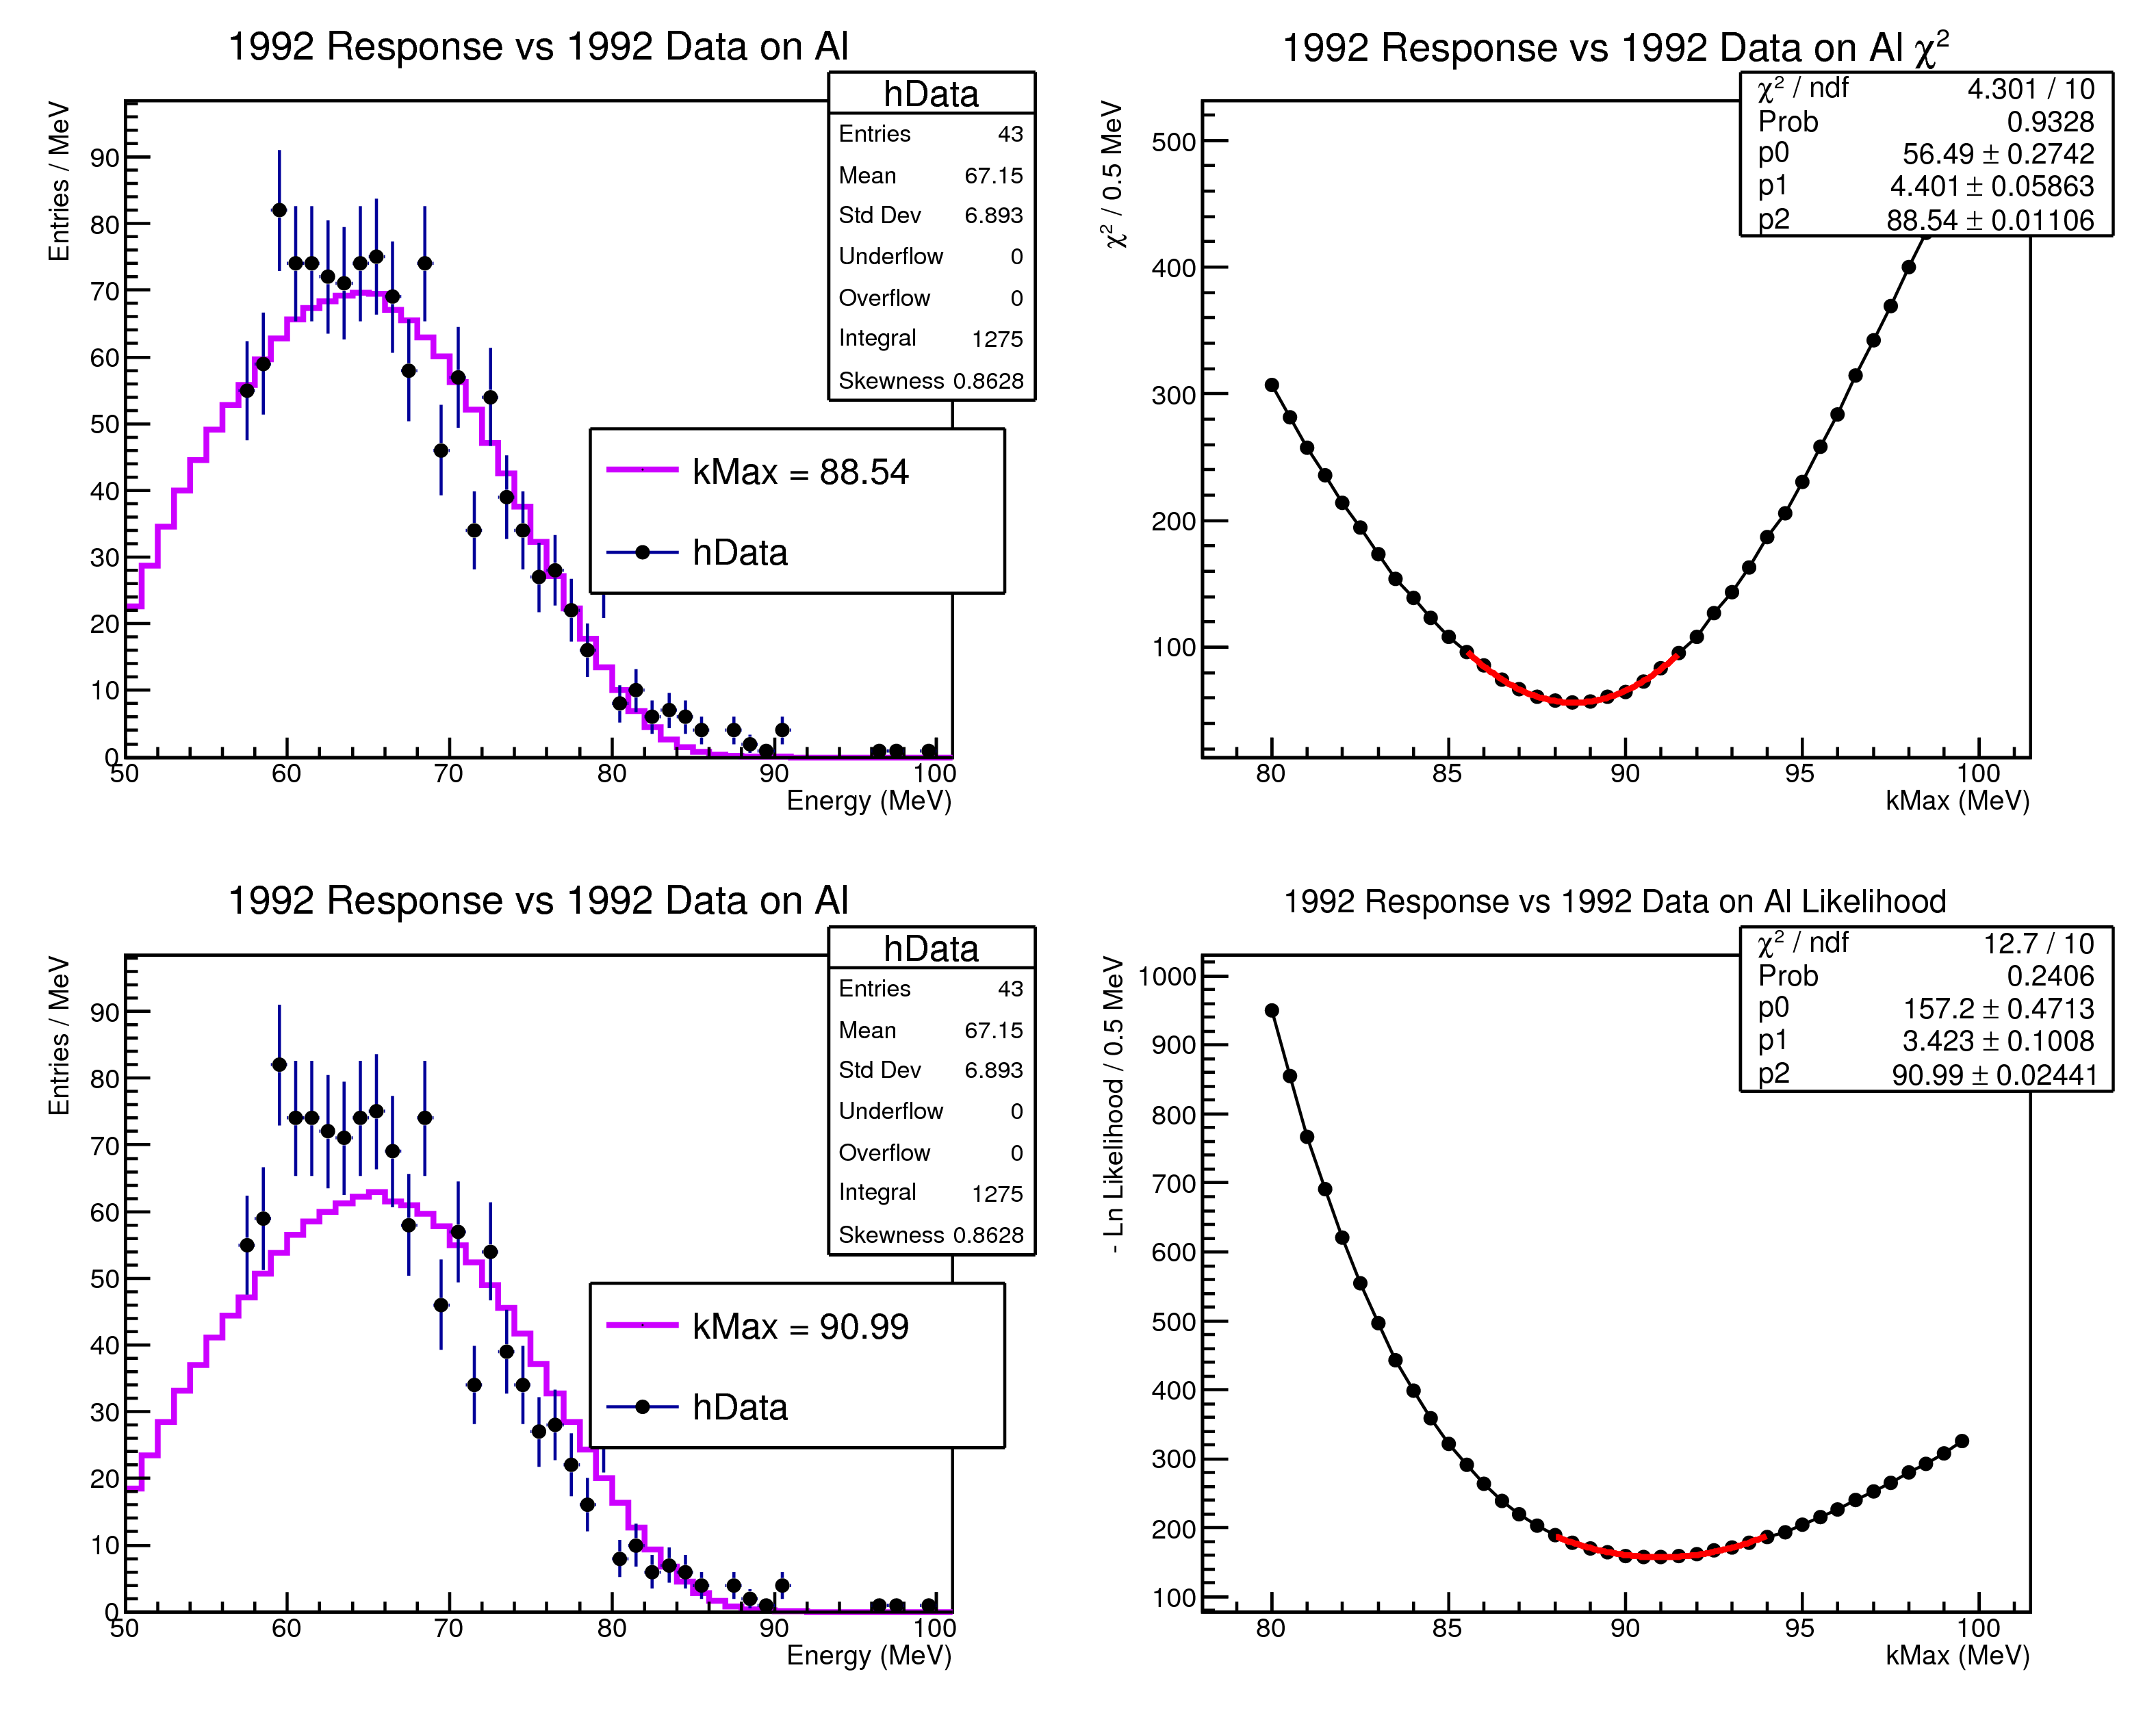
\includegraphics[width=0.8\linewidth]{figures/png/1992_resp_1992_Al_data_allPlots_singleK.png}
  \caption{The left figures show the best fit convolved closure approximation spectrum. The right figures
  show the parabolic fit to find the best fit endpoint energy. The top figures use $\chi ^2$ 
  minimization while the bottom figures use $\mathcal{L}$ minimization.}
  \label{fig:1992AlFits}
\end{figure}


\begin{figure}[h]
  \centering
  \subfloat[ $\chi^2$ Minimization Fit \label{fig:ChiSq}]{%
  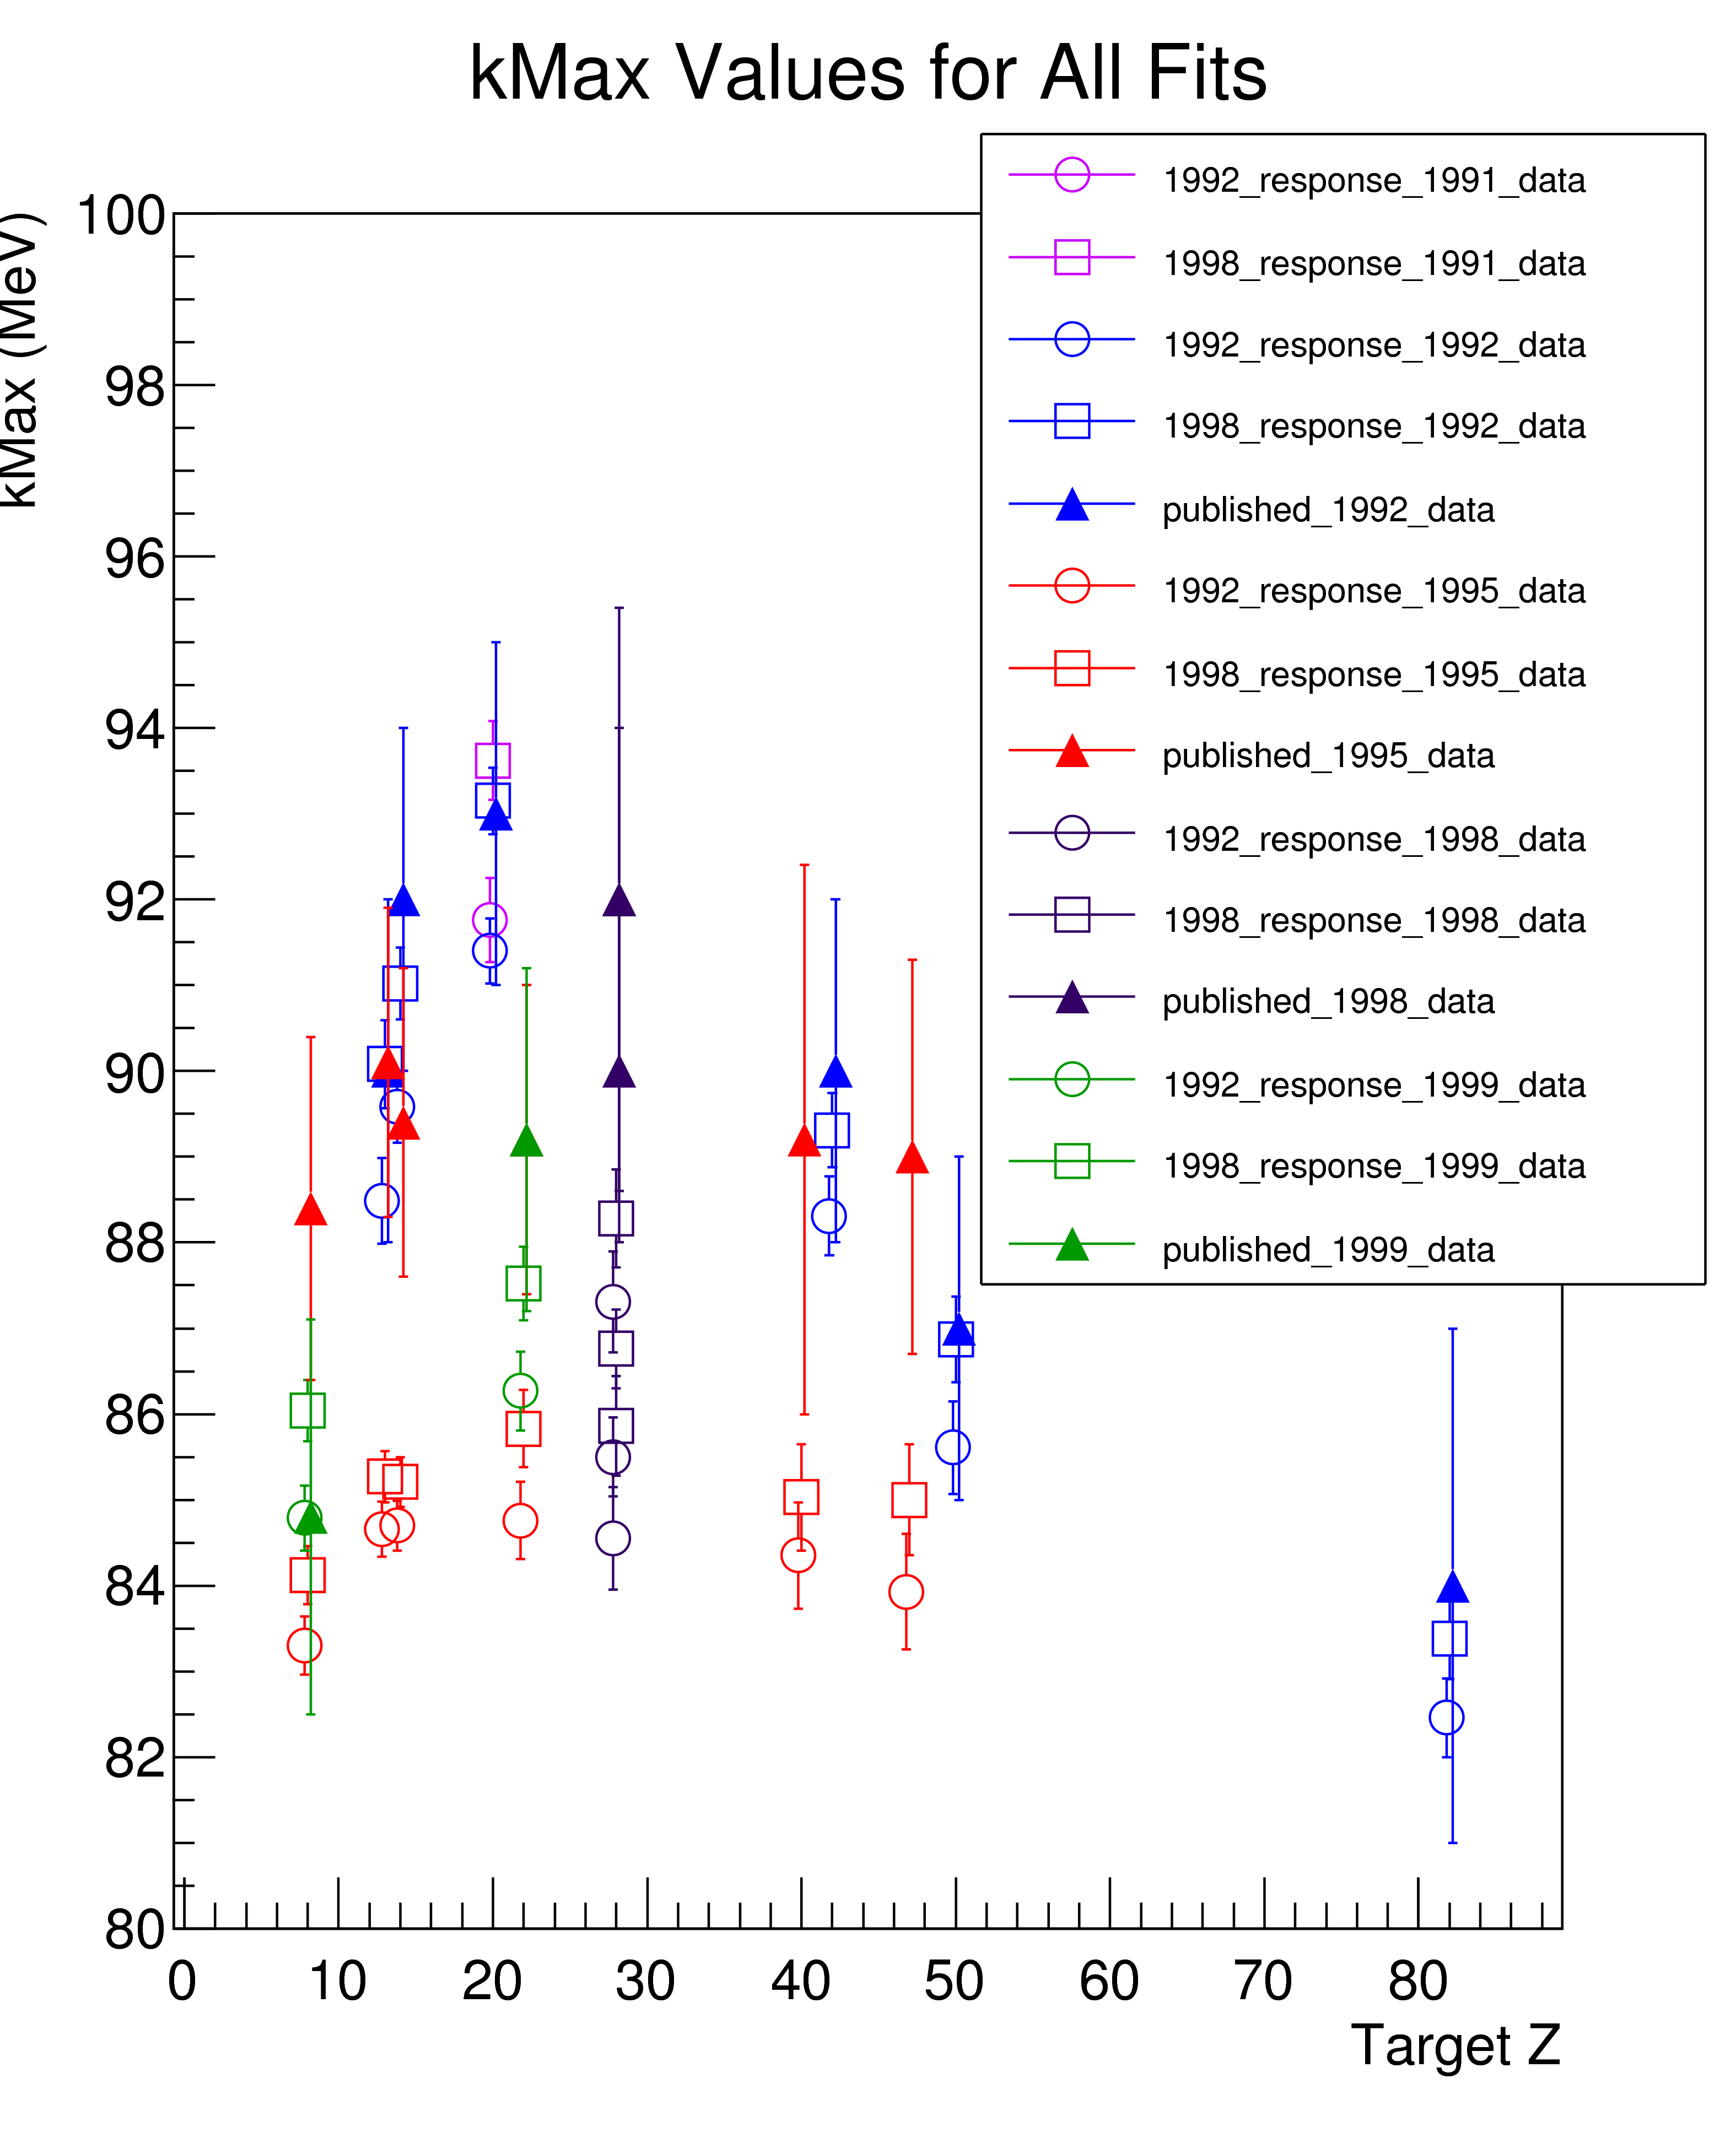
\includegraphics[width=0.48\linewidth]{figures/png/all_kMaxesChiSq_vs_target_z.png}
  }
  \hfill
  \subfloat[$\mathcal{L}$ Minimization Fit  \label{fig:NLL}]{%
  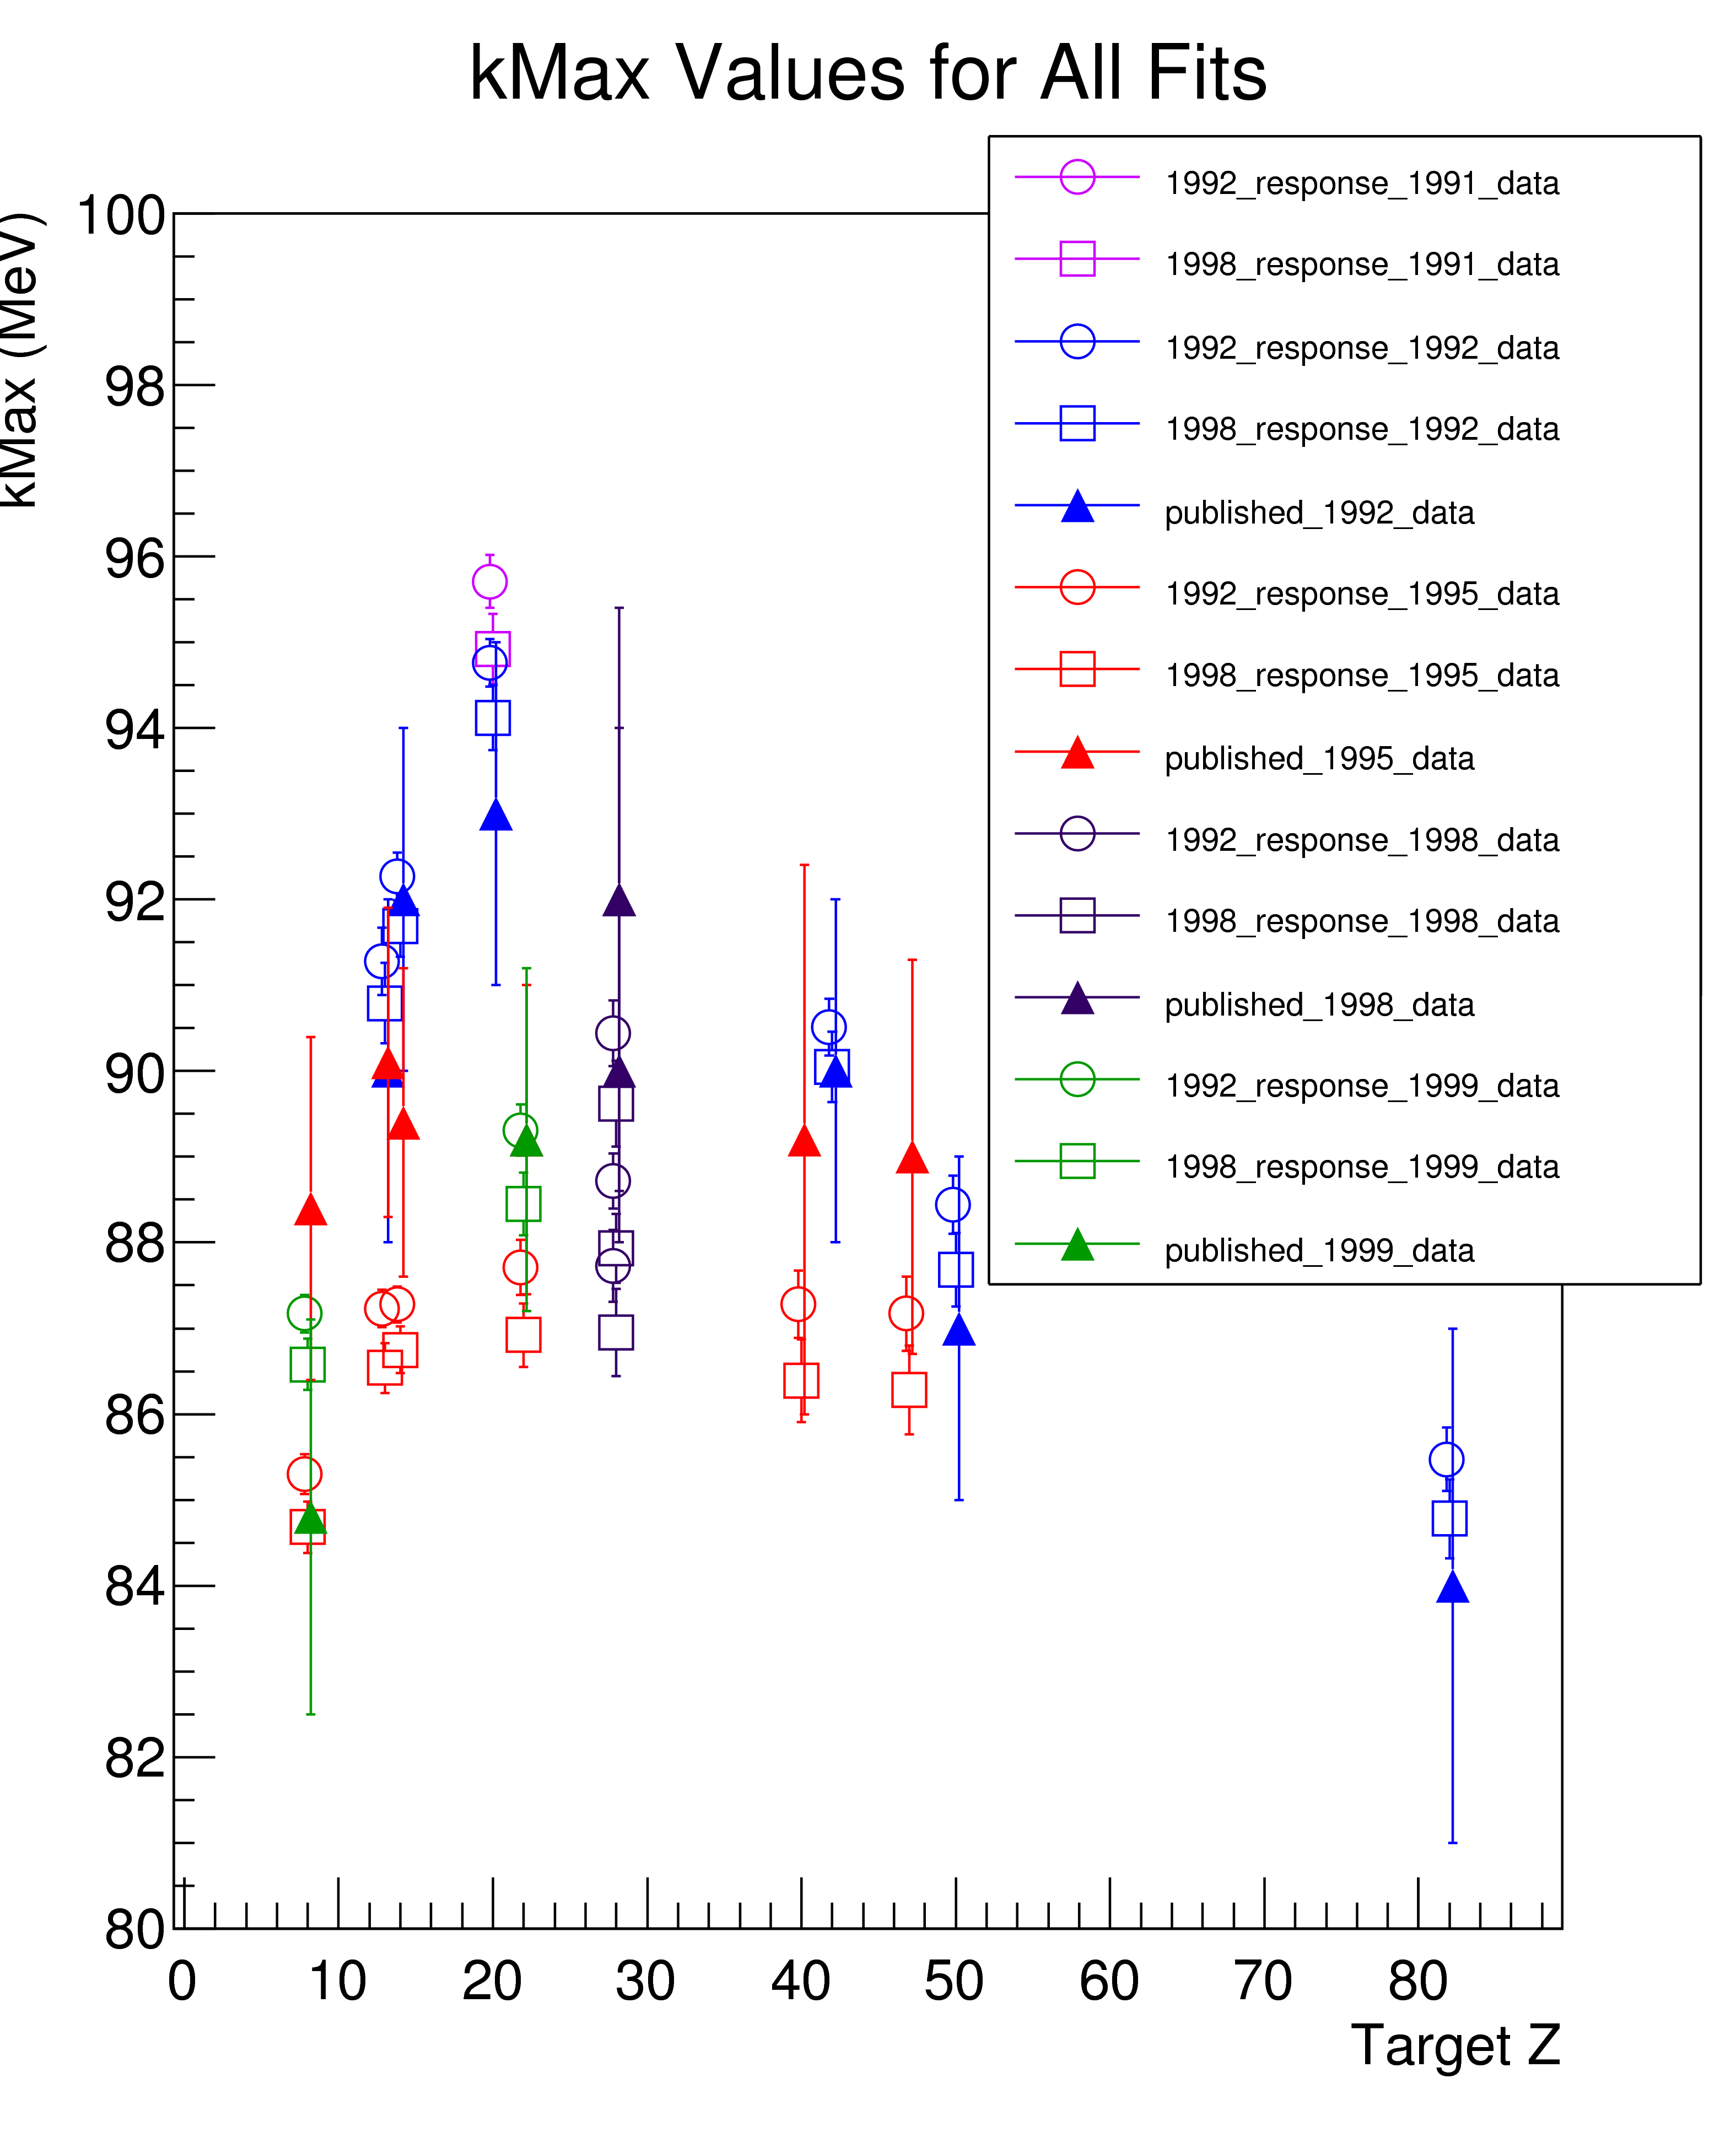
\includegraphics[width=0.48\linewidth]{figures/png/all_kMaxesNLL_vs_target_z.png}
  }
  \caption{Fit results vs target Z using (a) $\chi^2$ minimization and (b) $\mathcal{L}$ minimization.
    The 1992 detector response function data points (circles) are offset by -0.2 in z and the published data points (triangles)
    are offset by +0.2 in z.
  }
\end{figure}

%%%%%%%%%%%%%%%%%%%%%%%%%%%%%%%%%%%%%%%%%%%%%%%%%%%%%%%%%%%%%%%%%%%%%%%%%%%%%%%%%%%%%%%%%%%%%%%%%%%%%%
%% Should we include the chi square of the NLL fits, if we're not sure how they're defined in ROOT? %%
%%%%%%%%%%%%%%%%%%%%%%%%%%%%%%%%%%%%%%%%%%%%%%%%%%%%%%%%%%%%%%%%%%%%%%%%%%%%%%%%%%%%%%%%%%%%%%%%%%%%%%

\begin{figure}[h]
  \centering
  \includegraphics[width=0.8\linewidth]{figures/png/chiSq_of_fits.png}
  \caption{Fit $\chi^2$ values for both detector response functions and both fitting methods. }
  \label{fig:ChiSqOfFits}
\end{figure}


\begin{figure}[h]
  \centering
  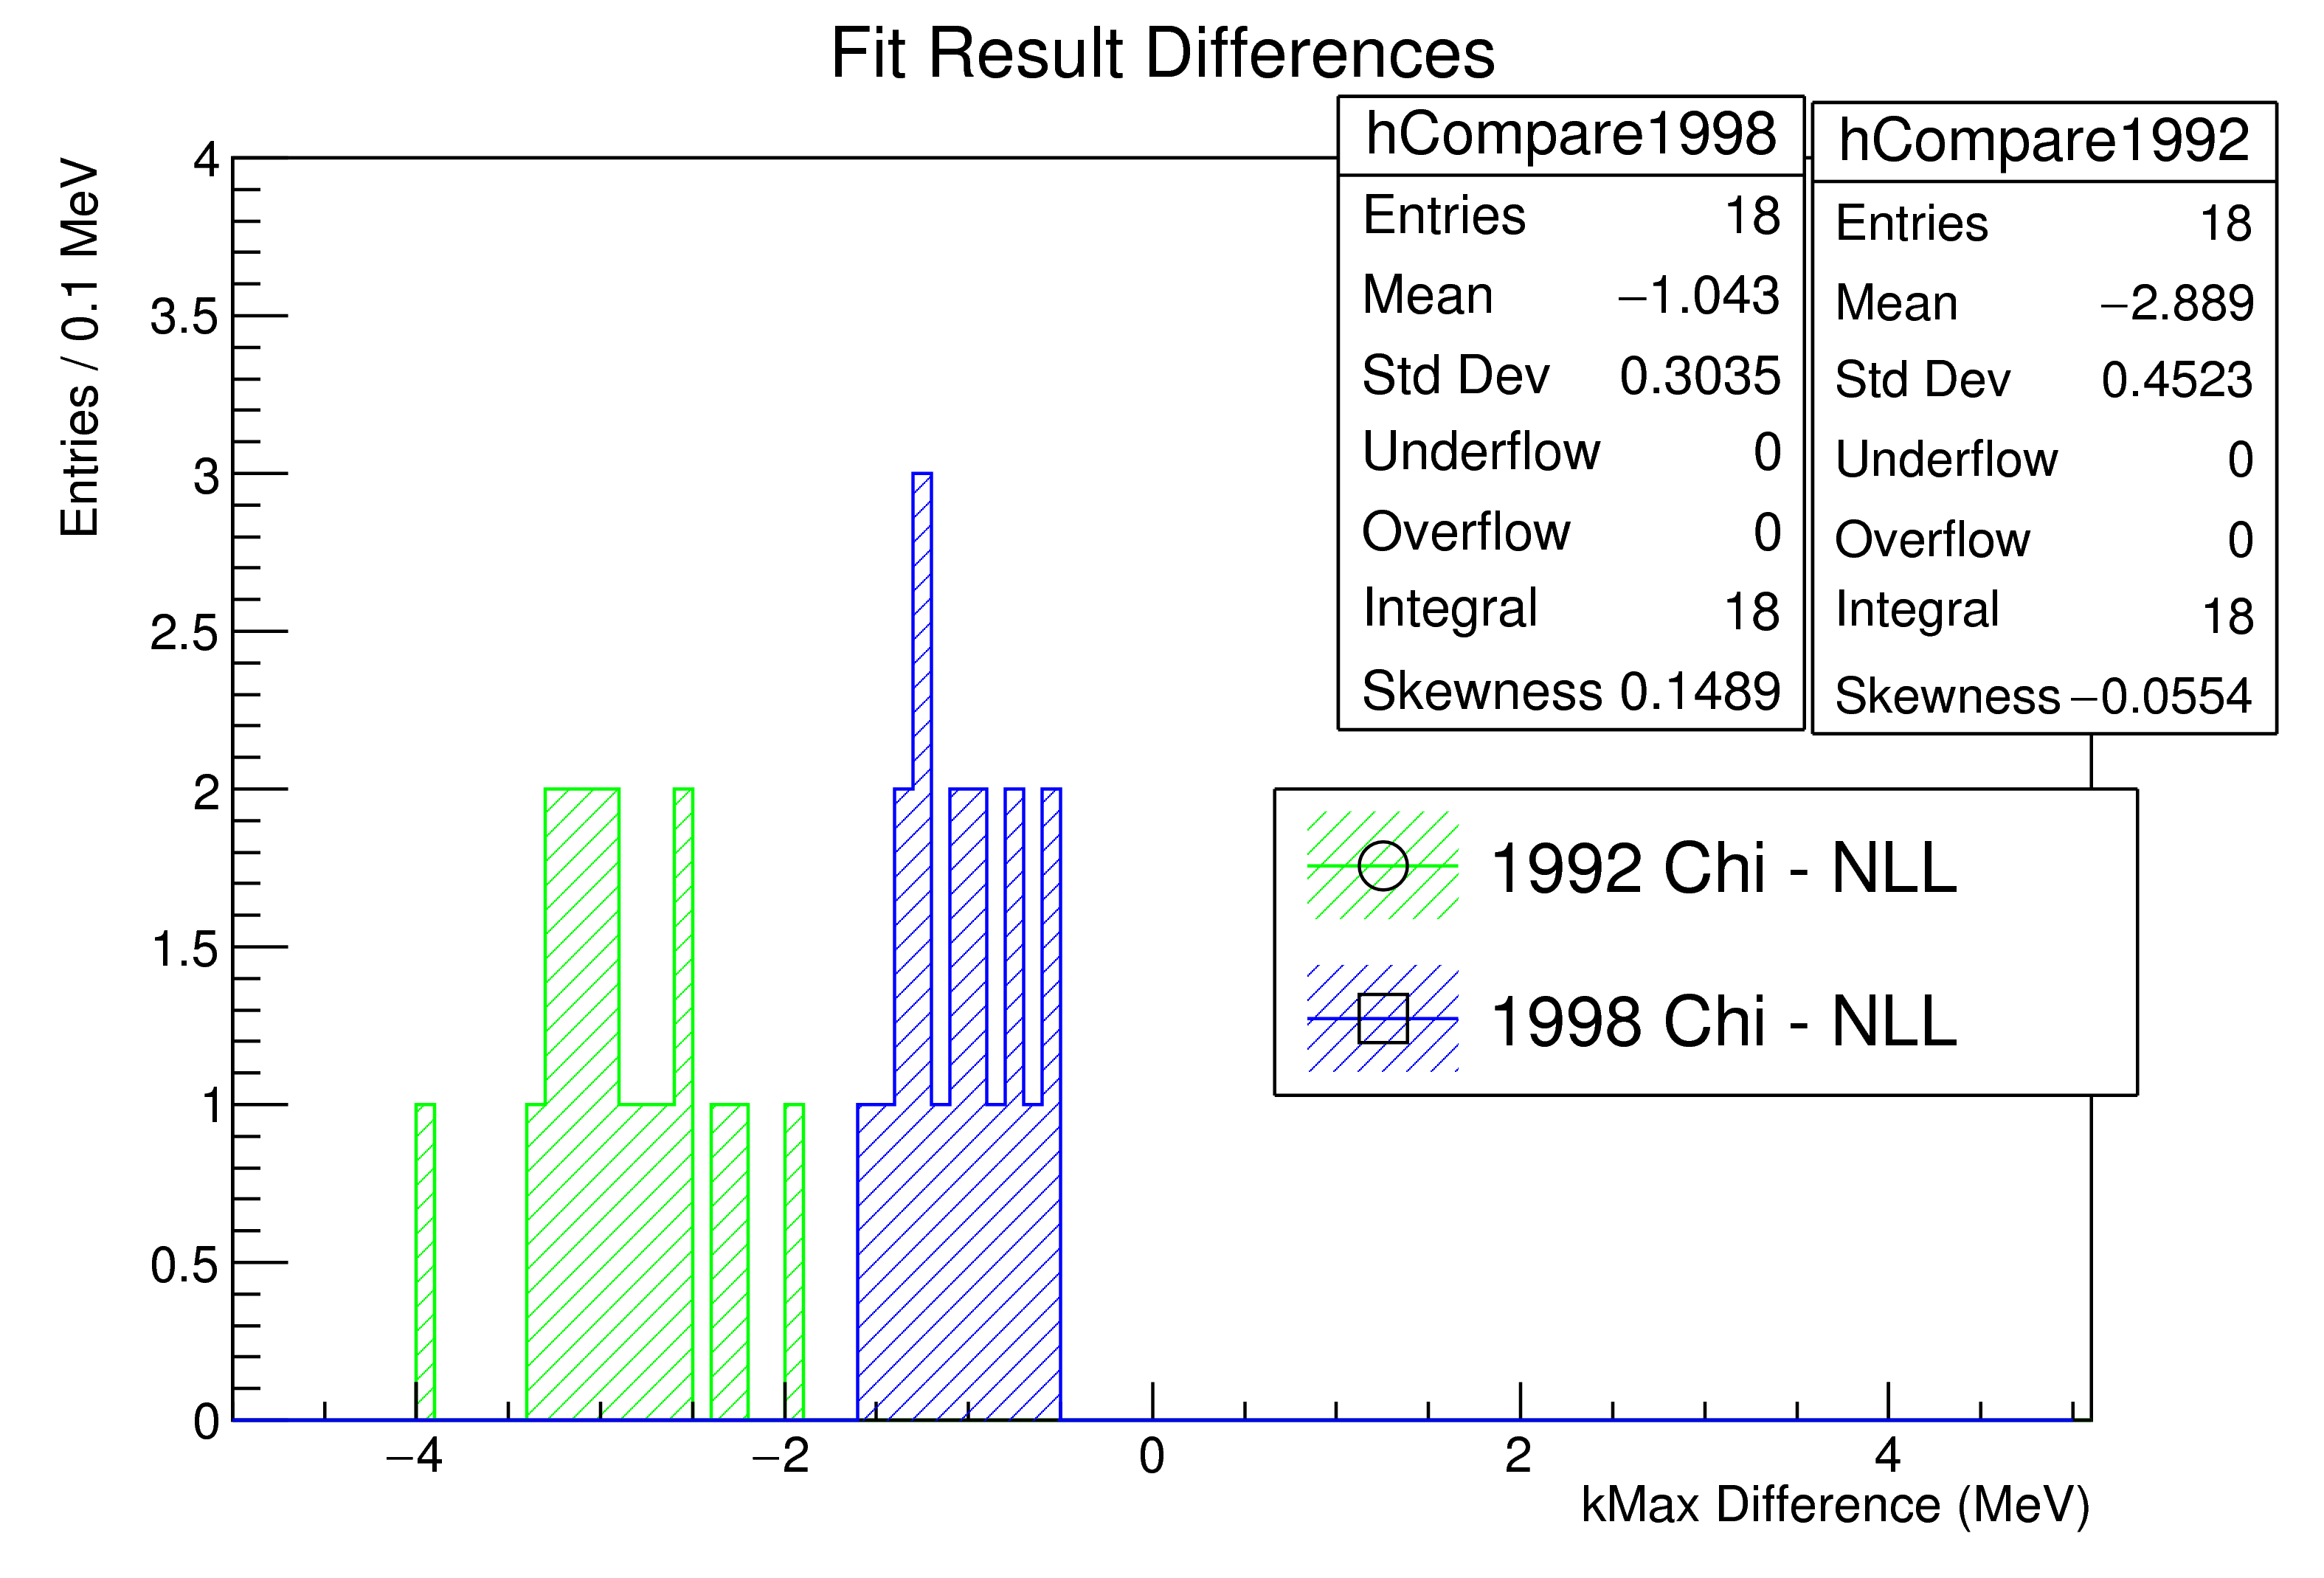
\includegraphics[width=\linewidth]{figures/png/compare_fit_results_92_v_98_unrestrictedOnly.png}
  \caption{The difference between the endpoint energies found using $\chi^2$ and
    $\mathcal{L}$ minimization using the 1992 and 1998 detector response functions.}
  \label{fig:compareFits}
\end{figure}

\begin{figure}[h]
  \centering
  \subfloat[ 1992 detector response \label{fig:1992ToyErrs}]{%
  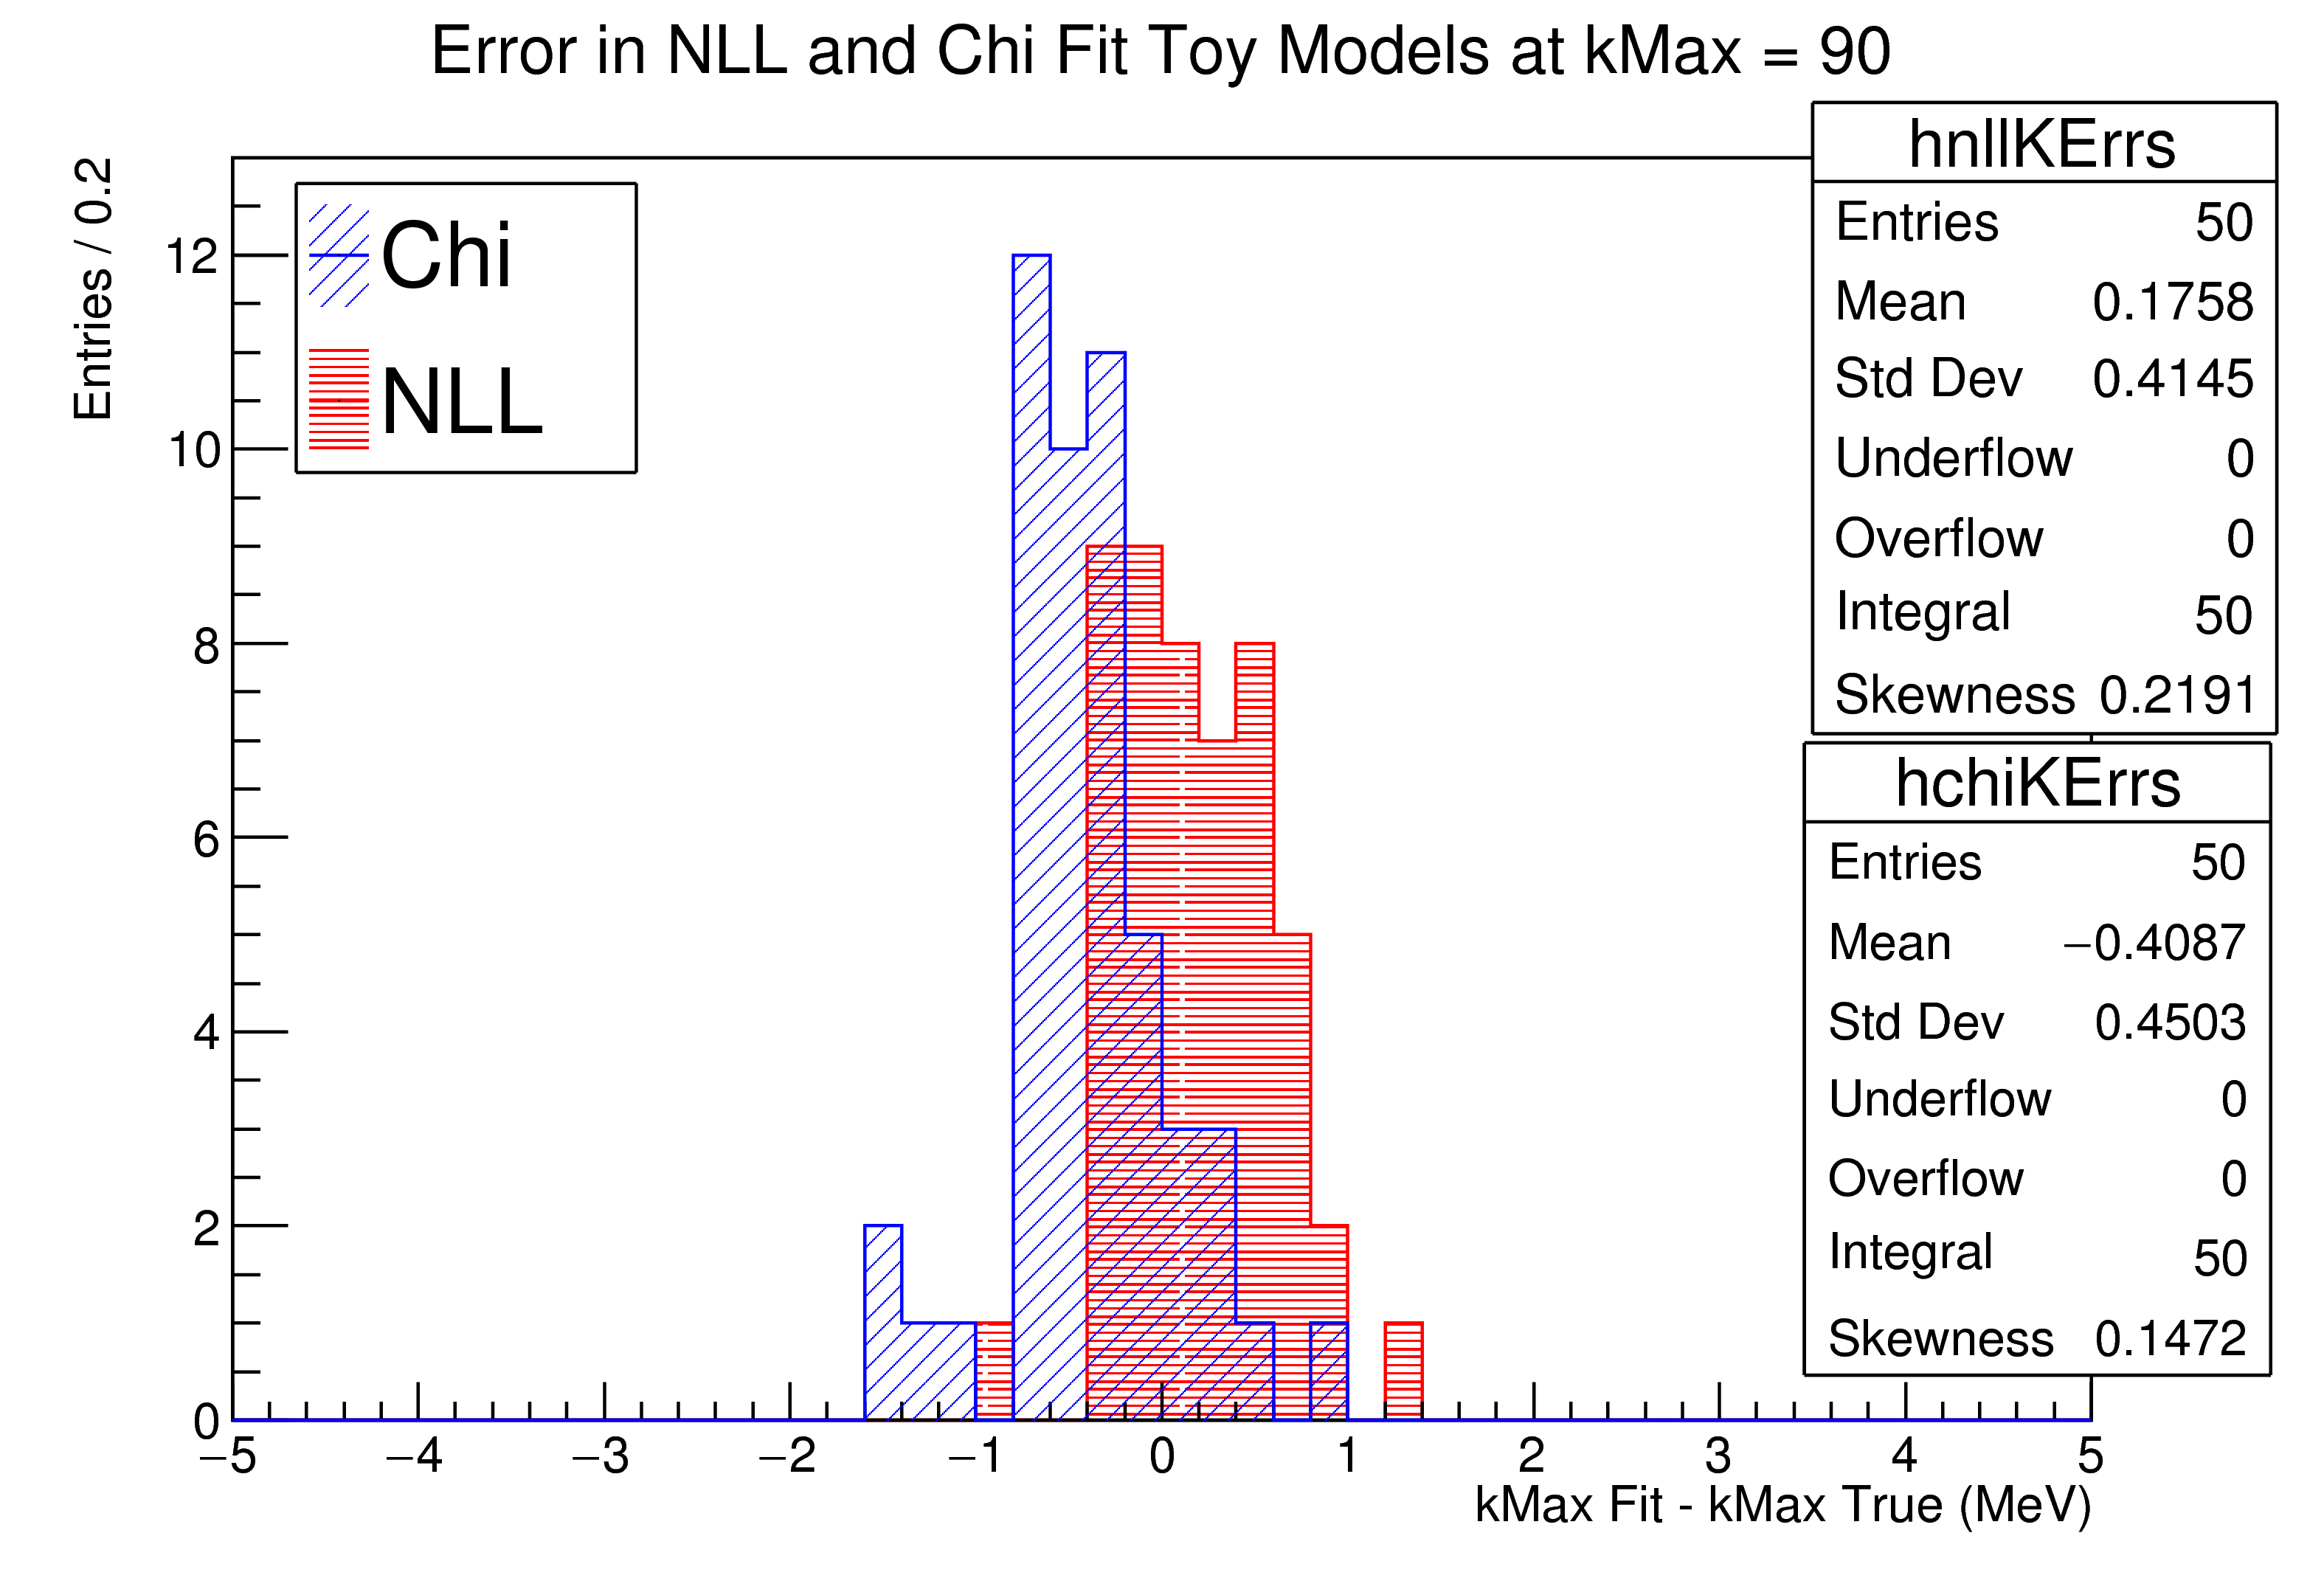
\includegraphics[width=0.48\linewidth]{figures/png/toy_kMax_errors_1992_response.png}
  }
  \hfill
  \subfloat[ 1998 detector response  \label{fig:1998ToyErrs}]{%
  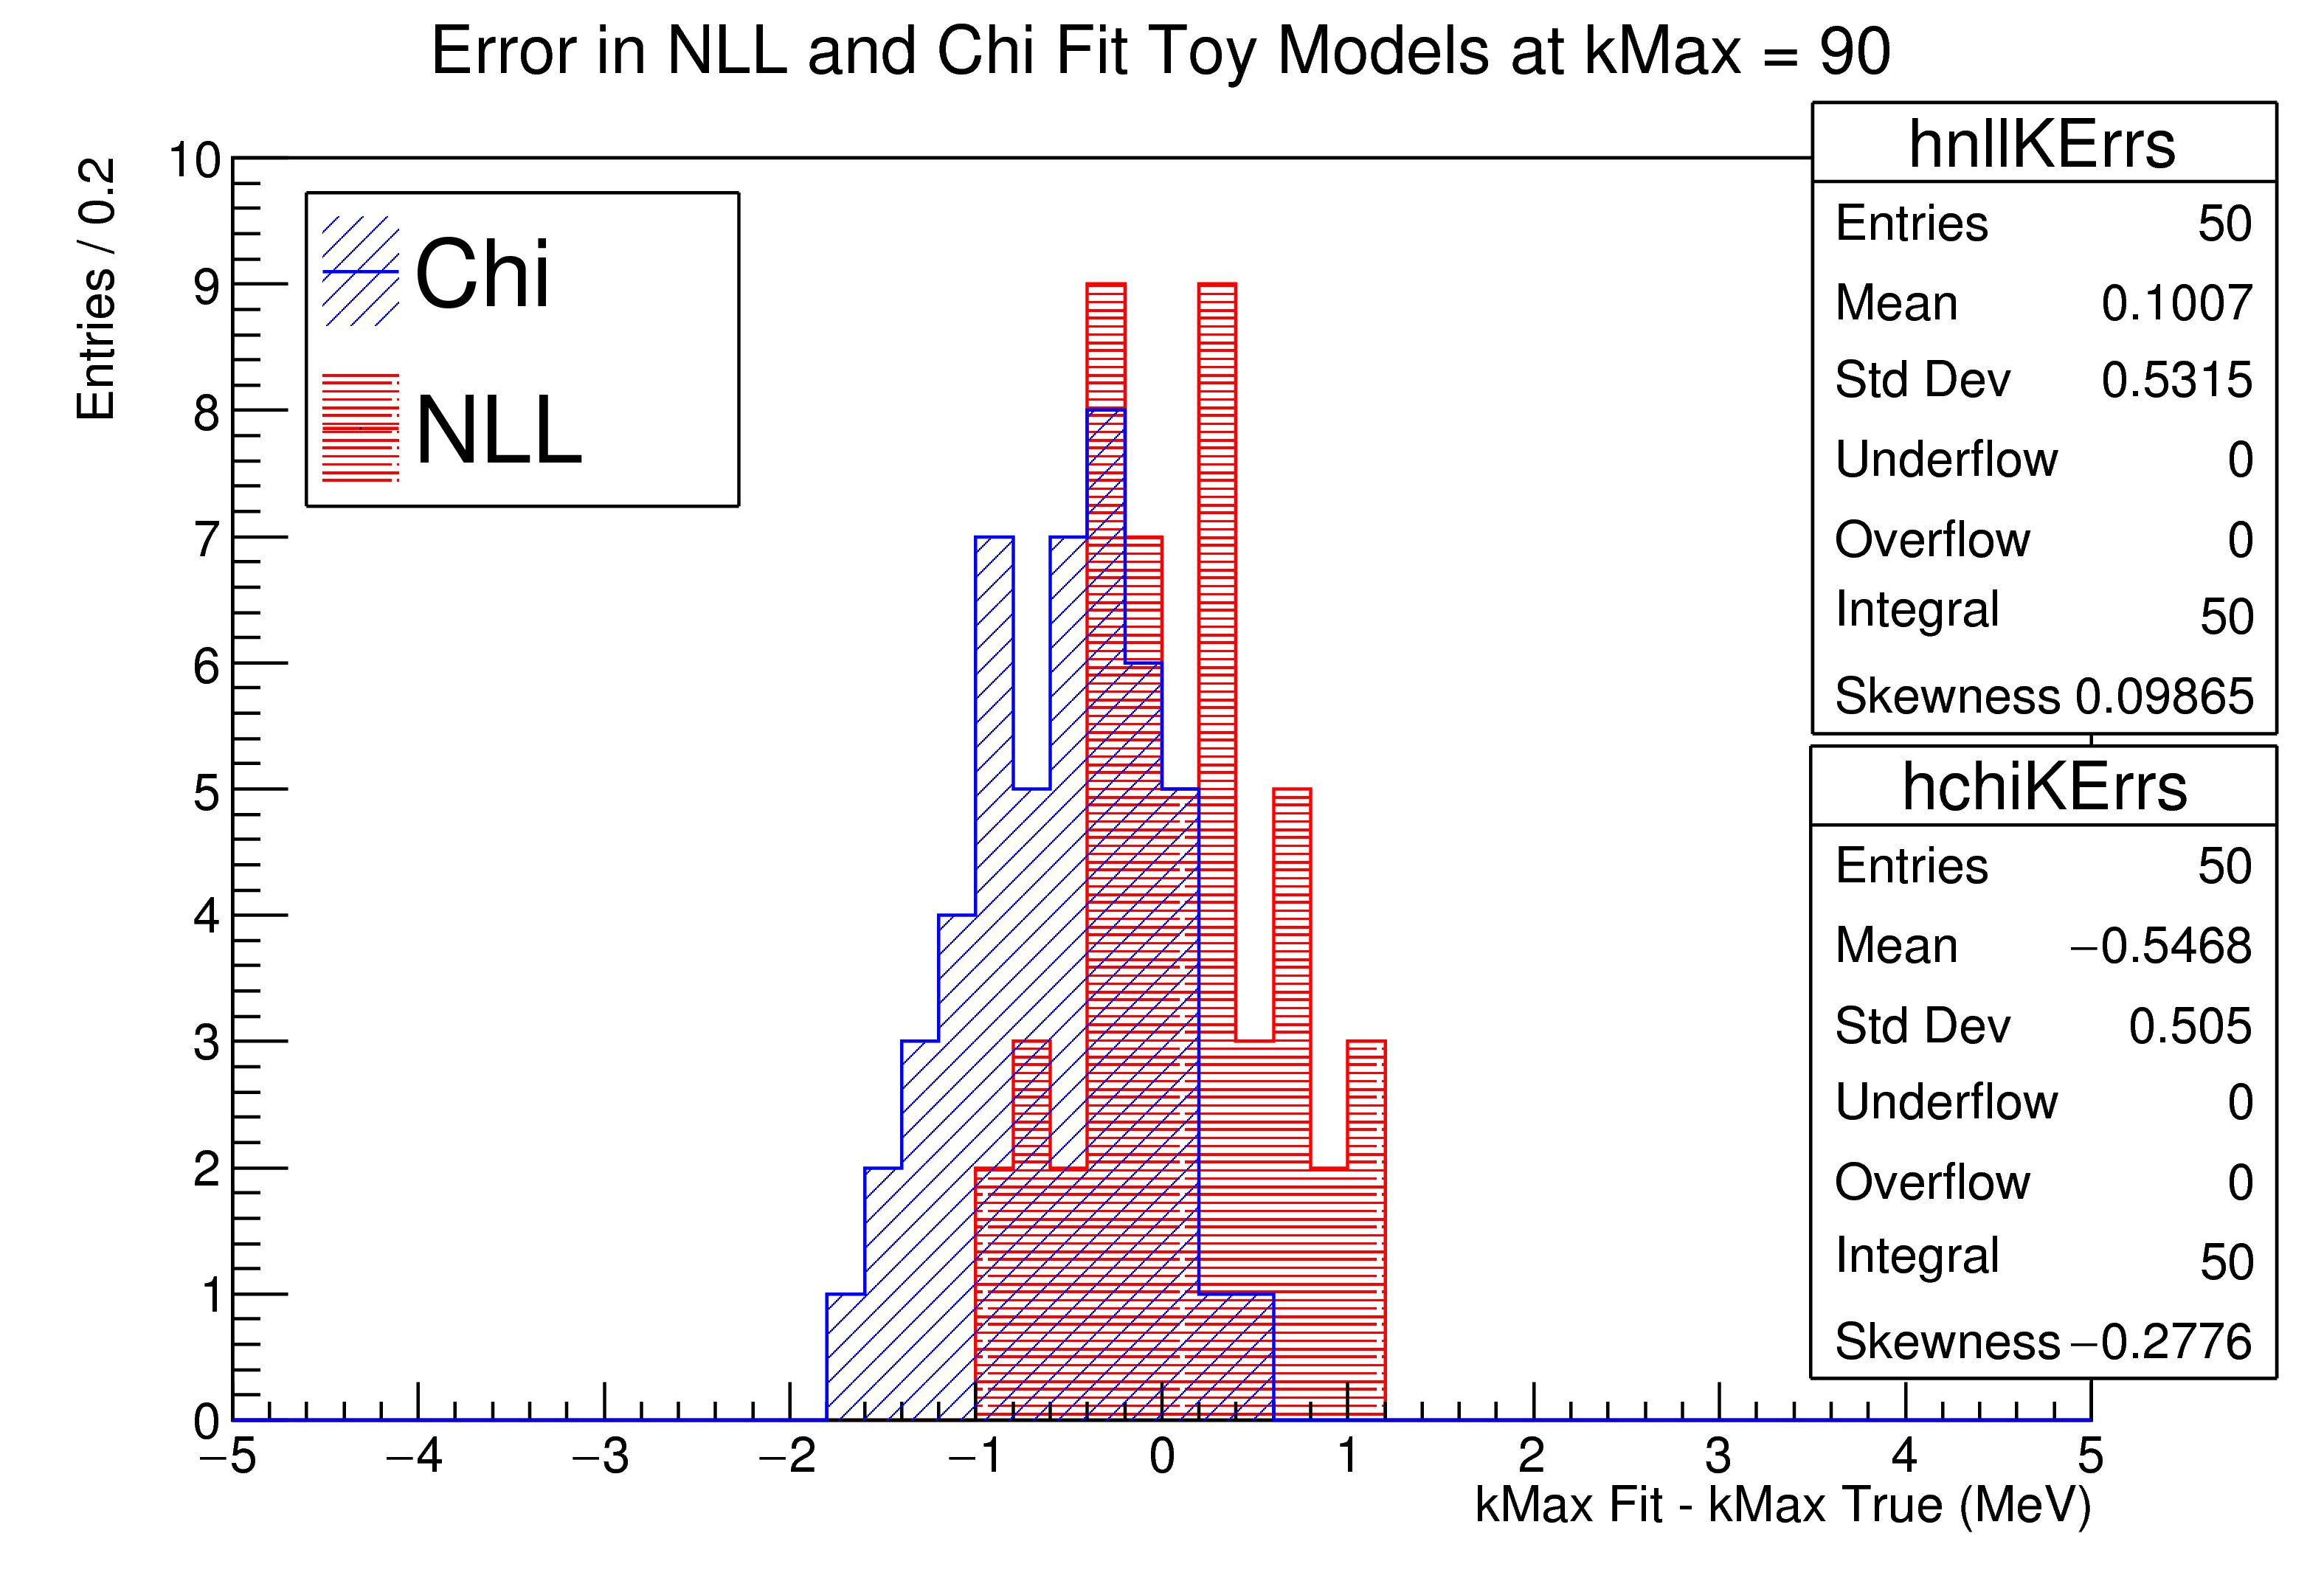
\includegraphics[width=0.48\linewidth]{figures/png/toy_kMax_errors_1998_response.png}
  }
  \caption{Fit results errors for 50 toy data sets using the (a) 1992 or (b) 1998 detector response function.
    The toy data sets are generated from a convolution with an endpoint energy of 90 MeV and generated
    with 1275 data points.
  }
  \label{fig:ToyFitErrs}
\end{figure}

\begin{figure}[h]
  \centering
  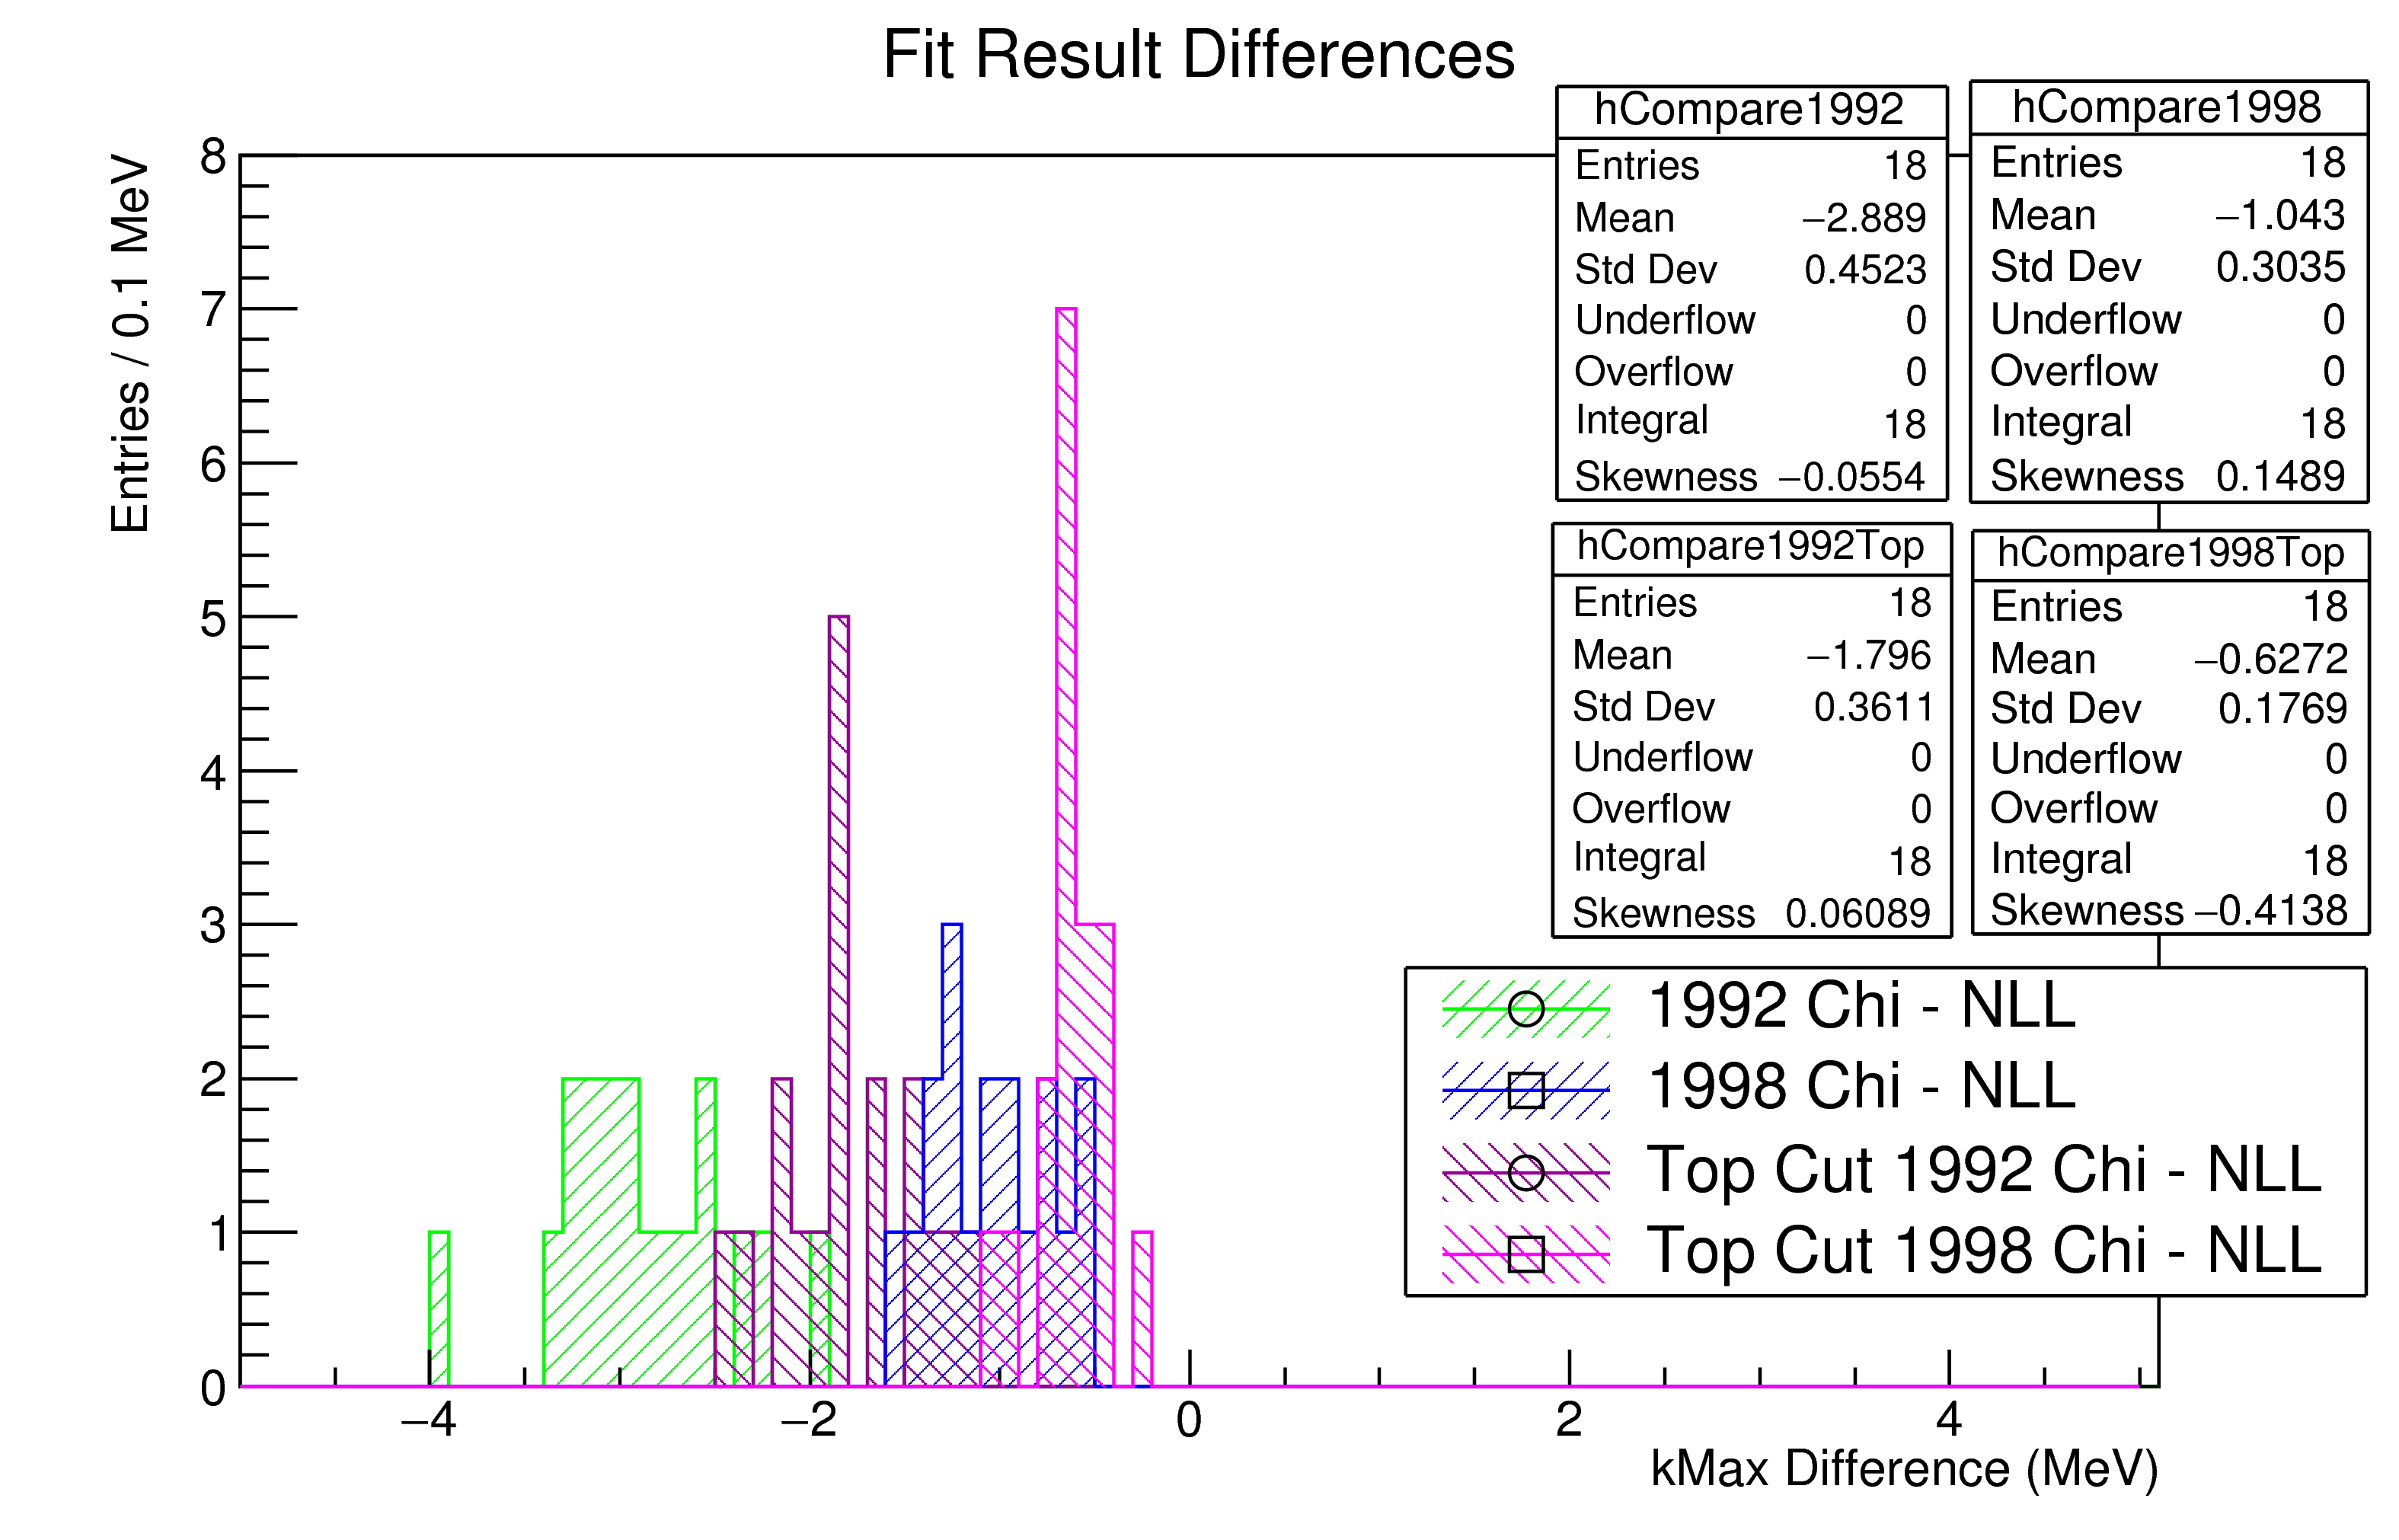
\includegraphics[width=\linewidth]{figures/png/compare_fit_results_92_v_98_with_topCut.png}
  \caption{The difference between the endpoint energies found using $\chi^2$ and
    $\mathcal{L}$ minimization with and without excluding the top 0.5\% of the data
    using the 1992 and 1998 detector response functions.}
  \label{fig:compareFitsTopCut}
\end{figure}


%% \begin{figure}[h]
%%   \centering
%%   \subfloat[ 1992 detector response \label{fig:1992ToyZs}]{%
%%   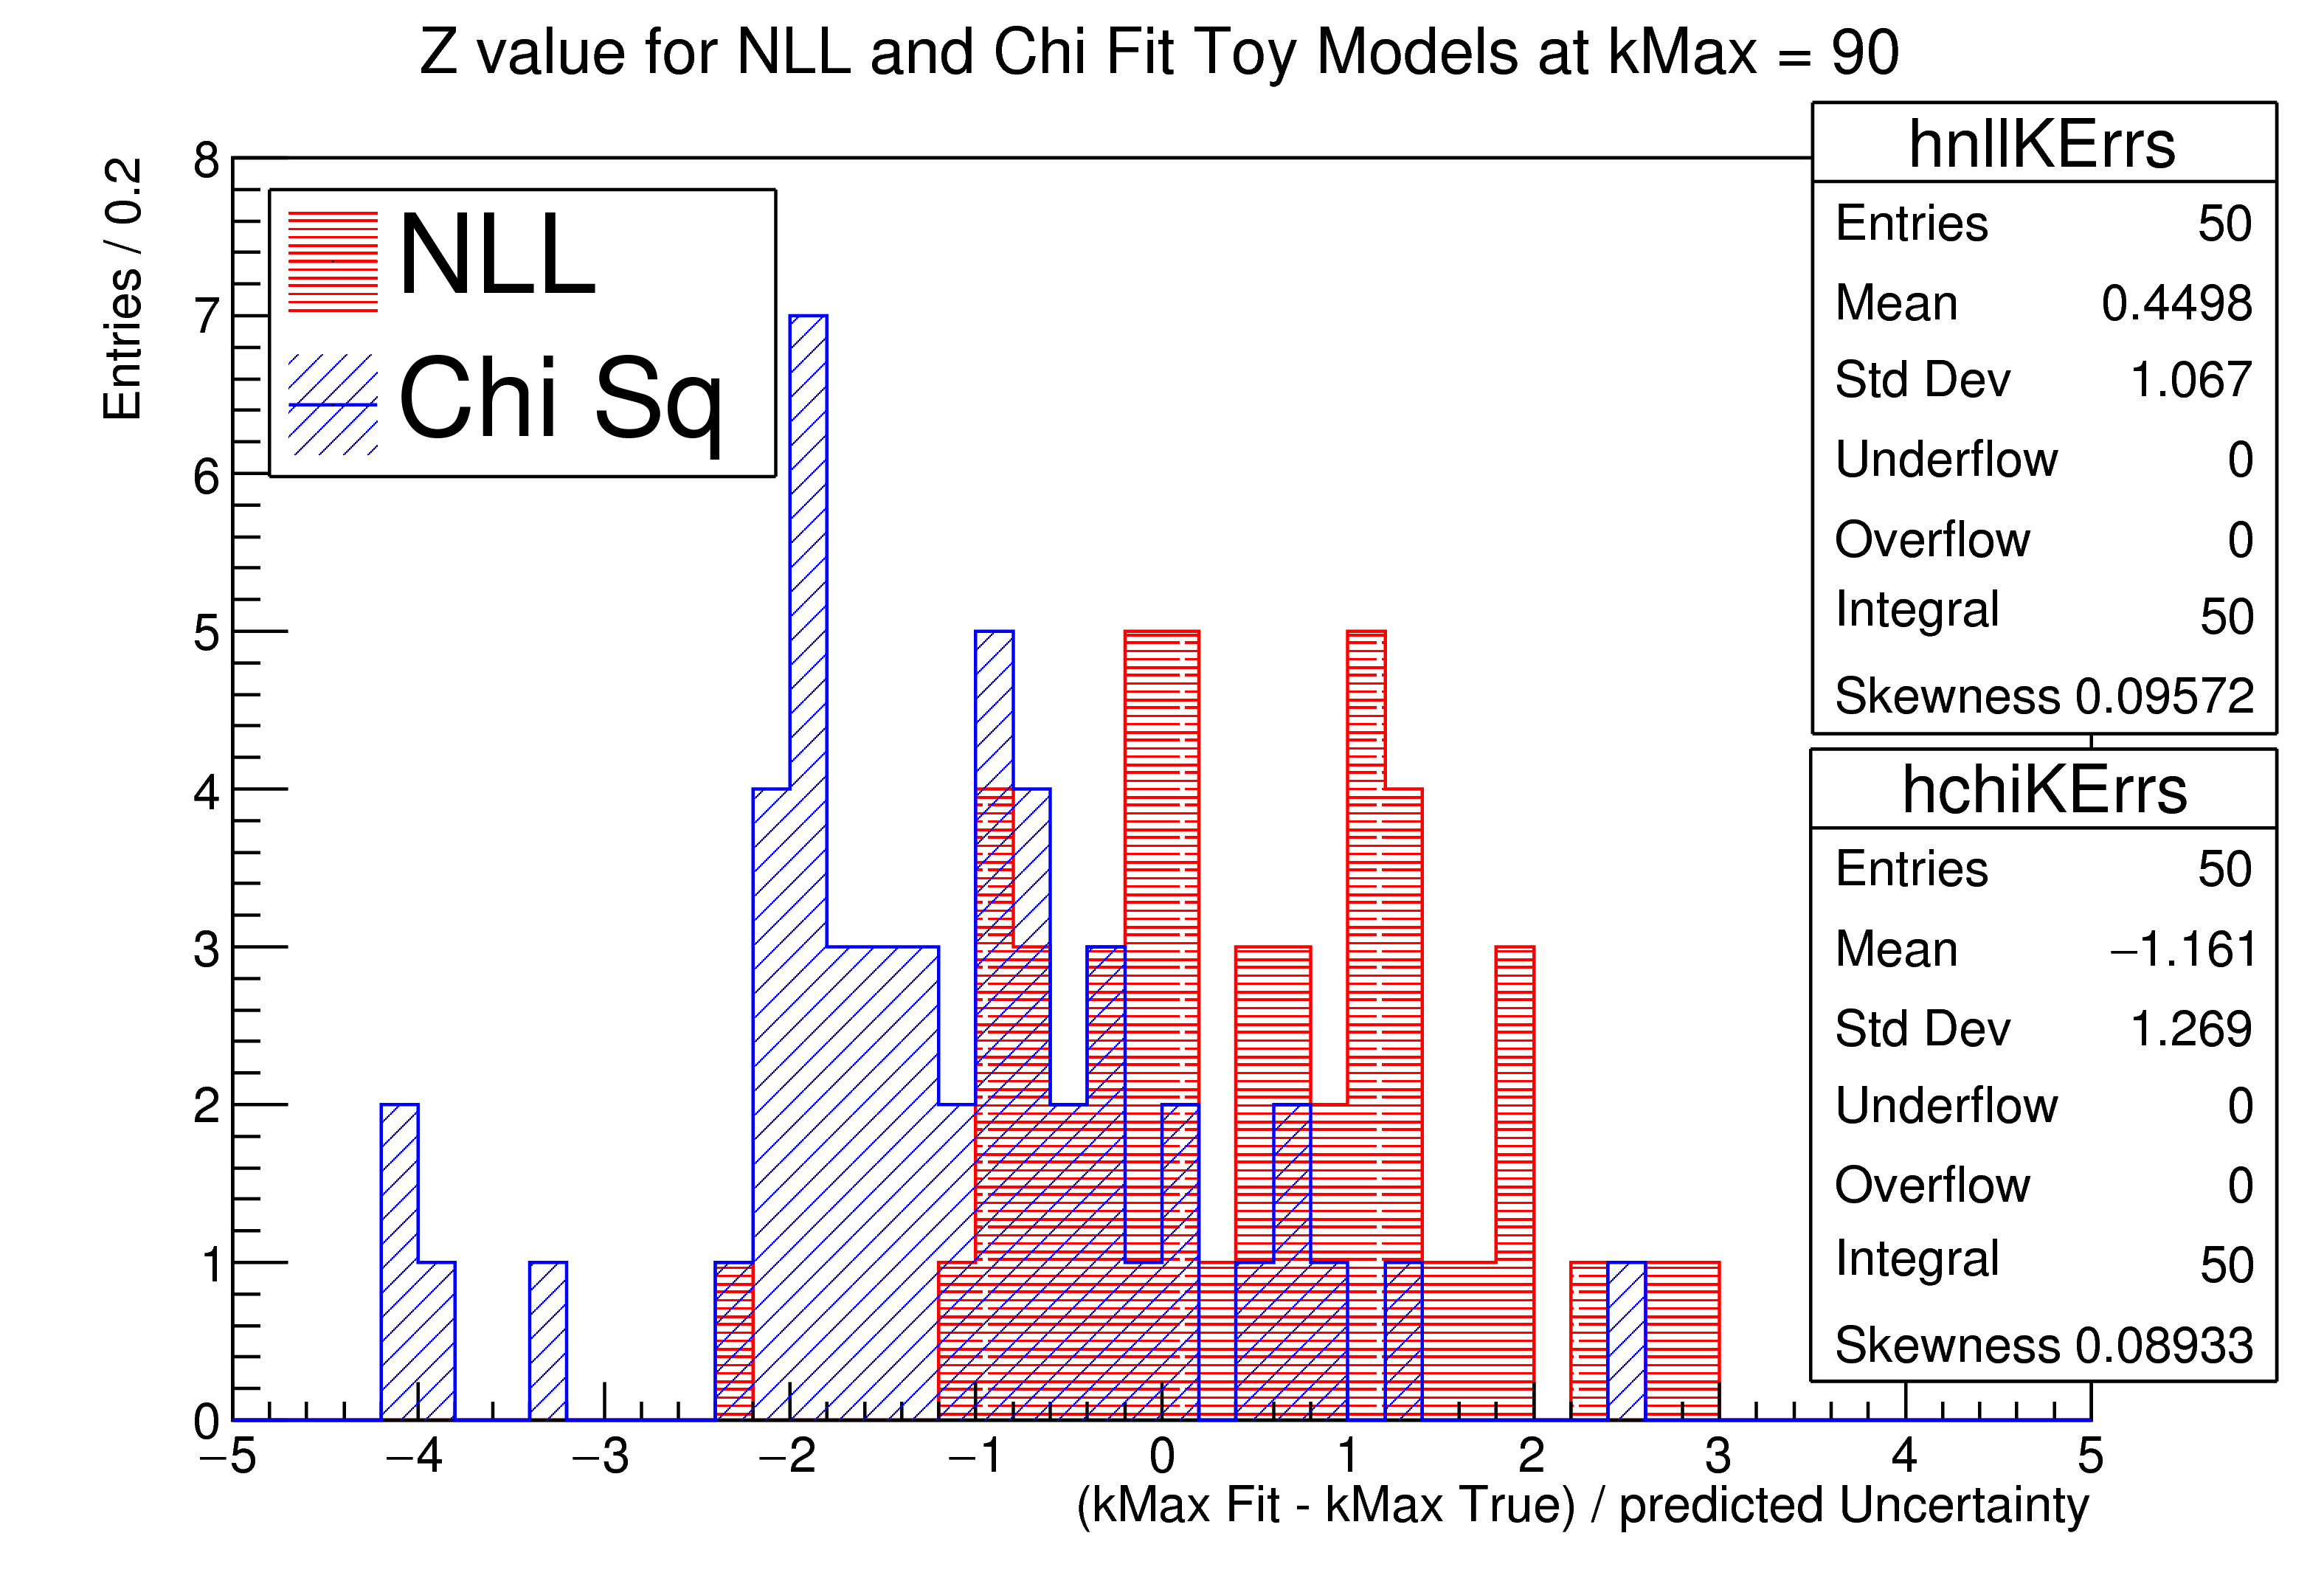
\includegraphics[width=0.48\linewidth]{figures/png/toy_kMax_z_values_1992_response.png}
%%   }
%%   \hfill
%%   \subfloat[ 1998 detector response  \label{fig:1998ToyZs}]{%
%%   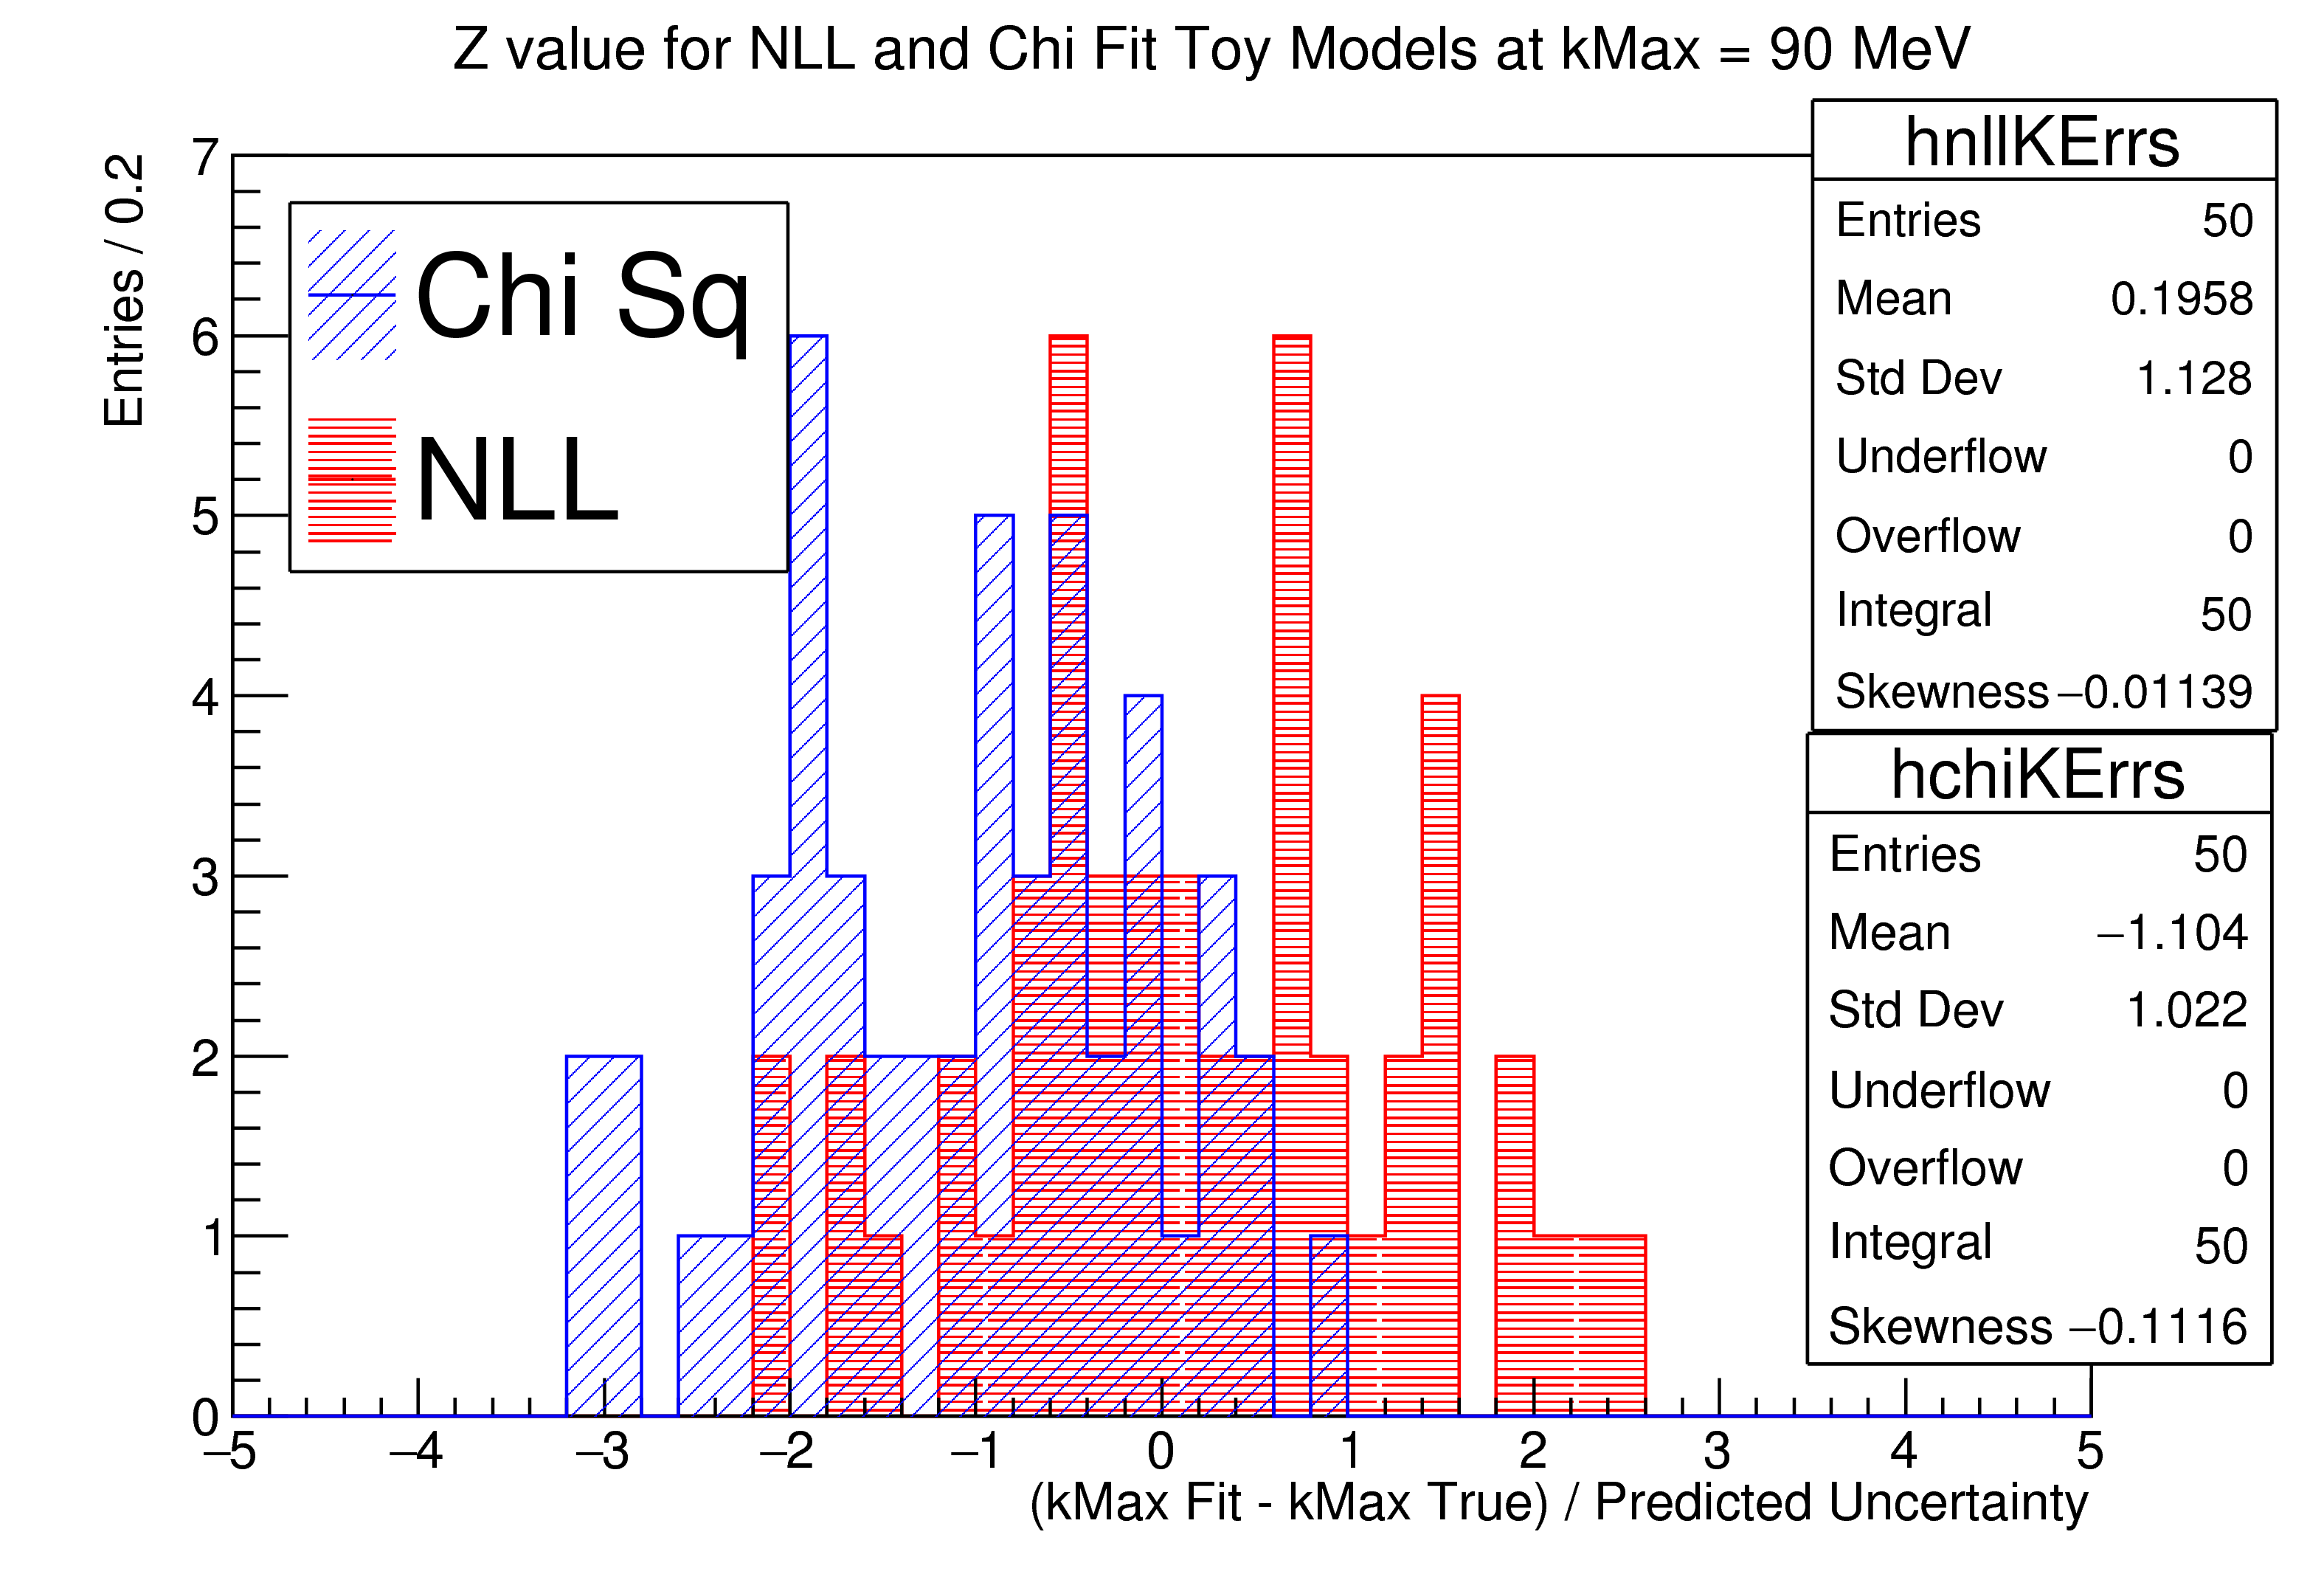
\includegraphics[width=0.48\linewidth]{figures/png/toy_kMax_z_values_1998_response.png}
%%   }
%%   \caption{Fit results z values for 50 toy data sets using the (a) 1992 or (b) 1998 detector response function.
%%     The toy data sets are generated from a convolution with an endpoint energy of 90 MeV and generated
%%     with 1275 data points. The z value for a fit is the fit endpoint value minus the true value, divided
%%     by the fit estimated uncertainty. 
%%   }
%%   \label{fig:ToyFitZs}
%% \end{figure}



%%%%%%%%%%%%%%%%%%%%%%%%%%%%%%%%%%%%%%%%%%%%%%%%%%%%%%%%%%%%%%%%%%%%%%%%%%%%%%

%% Year, Target, Response, chiKMax, chiKErr, chiChi, chiDoF, chiChiDoF, nllChi, nllDoF, nllChiDoF, nllkMax, nllkErr: 1992 Al 1992 88.5653 0.4781 49.8284 30 1.6609 65.8355 33 1.9950 90.1736 0.3638      
%% Year, Target, Response, chiKMax, chiKErr, chiChi, chiDoF, chiChiDoF, nllChi, nllDoF, nllChiDoF, nllkMax, nllkErr: 1992 Al 1998 89.9455 0.5029 35.5187 30 1.1840 50.6788 33 1.5357 90.2135 0.5014

%% Year, Target, Response, chiKMax, chiKErr, chiChi, chiDoF, chiChiDoF, nllChi, nllDoF, nllChiDoF, nllkMax, nllkErr: 1992 Ca 1992 91.3949 0.3781 87.3362 33 2.6465 131.9163 35 3.7690 93.7088 0.2757     
%% Year, Target, Response, chiKMax, chiKErr, chiChi, chiDoF, chiChiDoF, nllChi, nllDoF, nllChiDoF, nllkMax, nllkErr: 1992 Ca 1998 93.2098 0.4125 45.1158 33 1.3672 51.0849 35 1.4596 93.7725 0.4219

%% Year, Target, Response, chiKMax, chiKErr, chiChi, chiDoF, chiChiDoF, nllChi, nllDoF, nllChiDoF, nllkMax, nllkErr: 1992 Mo 1992 88.3599 0.4477 42.1539 28 1.5055 47.0123 30 1.5671 89.5085 0.3358      
%% Year, Target, Response, chiKMax, chiKErr, chiChi, chiDoF, chiChiDoF, nllChi, nllDoF, nllChiDoF, nllkMax, nllkErr: 1992 Mo 1998 89.3734 0.4540 21.9226 28 0.7830 21.4937 30 0.7165 89.9247 0.4723

%% Year, Target, Response, chiKMax, chiKErr, chiChi, chiDoF, chiChiDoF, nllChi, nllDoF, nllChiDoF, nllkMax, nllkErr: 1992 Pb 1992 82.4471 0.4909 36.4359 26 1.4014 55.4372 28 1.9799 84.4161 0.3437      
%% Year, Target, Response, chiKMax, chiKErr, chiChi, chiDoF, chiChiDoF, nllChi, nllDoF, nllChiDoF, nllkMax, nllkErr: 1992 Pb 1998 83.3678 0.4724 14.3757 26 0.5529 17.5436 28 0.6266 84.0616 0.4588

%% Year, Target, Response, chiKMax, chiKErr, chiChi, chiDoF, chiChiDoF, nllChi, nllDoF, nllChiDoF, nllkMax, nllkErr: 1992 Si 1992 89.5762 0.4200 92.0027 30 3.0668 112.0776 32 3.5024 91.4077 0.3009     
%% Year, Target, Response, chiKMax, chiKErr, chiChi, chiDoF, chiChiDoF, nllChi, nllDoF, nllChiDoF, nllkMax, nllkErr: 1992 Si 1998 90.9247 0.4138 39.2309 30 1.3077 41.5799 32 1.2994 91.5952 0.4064

%% Year, Target, Response, chiKMax, chiKErr, chiChi, chiDoF, chiChiDoF, nllChi, nllDoF, nllChiDoF, nllkMax, nllkErr: 1992 Sn 1992 85.6288 0.5288 68.1821 26 2.6224 84.2806 28 3.0100 87.5107 0.3406      
%% Year, Target, Response, chiKMax, chiKErr, chiChi, chiDoF, chiChiDoF, nllChi, nllDoF, nllChiDoF, nllkMax, nllkErr: 1992 Sn 1998 87.0685 0.5266 19.3492 26 0.7442 21.1440 28 0.7551 87.4817 0.4789


\subsection { Fits of the 1992 data }
\begin{table}[h]
  \begin{center}
    \begin{tabular}{|l||l|l|l|l|l|l|}
      \hline
      Dataset & Published $k_{Max}$ & $\chi^2 / DoF$ & Our $k_{Max}$ & $\chi^2 / DoF$  & Response & Fit \\
      \hhline{|=||=|=|=|=|=|=|}
      Al 1992 & 90   $\pm$ 2   & 1.1 & 88.6 $\pm$ 0.5 & 1.7 ( 49.8 / 30) & 1992 & $\chi^2$      \\
      Al 1992 &                &     & 89.9 $\pm$ 0.5 & 1.2 ( 35.5 / 30) & 1998 & $\chi^2$      \\
      Al 1992 &                &     & 90.2 $\pm$ 0.4 & 2.0 ( 65.8 / 33) & 1992 & $\mathcal{L}$ \\
      Al 1992 &                &     & 90.2 $\pm$ 0.5 & 1.5 ( 50.7 / 33) & 1998 & $\mathcal{L}$ \\
      \hline                                                                                    
      Ca 1992 & 93   $\pm$ 2   & 1.6 & 91.4 $\pm$ 0.4 & 2.7 ( 87.3 / 33) & 1992 & $\chi^2$      \\
      Ca 1992 &                &     & 93.2 $\pm$ 0.4 & 1.4 ( 45.1 / 33) & 1998 & $\chi^2$      \\
      Ca 1992 &                &     & 93.7 $\pm$ 0.3 & 3.8 (131.9 / 35) & 1992 & $\mathcal{L}$ \\
      Ca 1992 &                &     & 93.8 $\pm$ 0.4 & 1.5 ( 51.1 / 35) & 1998 & $\mathcal{L}$ \\
      \hline                                                                                    
      Mo 1992 & 90   $\pm$ 2   & 0.8 & 88.4 $\pm$ 0.5 & 1.5 ( 42.2 / 28) & 1992 & $\chi^2$      \\
      Mo 1992 &                &     & 89.4 $\pm$ 0.5 & 0.8 ( 21.9 / 28) & 1998 & $\chi^2$      \\
      Mo 1992 &                &     & 89.5 $\pm$ 0.3 & 1.6 ( 47.0 / 30) & 1992 & $\mathcal{L}$ \\
      Mo 1992 &                &     & 89.9 $\pm$ 0.5 & 0.7 ( 21.5 / 30) & 1998 & $\mathcal{L}$ \\
      \hline                                                                                    
      Pb 1992 & 84   $\pm$ 3   & 0.9 & 82.4 $\pm$ 0.5 & 1.4 ( 36.4 / 26) & 1992 & $\chi^2$      \\
      Pb 1992 &                &     & 83.4 $\pm$ 0.5 & 0.6 ( 14.4 / 26) & 1998 & $\chi^2$      \\
      Pb 1992 &                &     & 84.4 $\pm$ 0.3 & 2.0 ( 55.4 / 28) & 1992 & $\mathcal{L}$ \\
      Pb 1992 &                &     & 84.1 $\pm$ 0.5 & 0.6 ( 17.5 / 28) & 1998 & $\mathcal{L}$ \\
      \hline                                                                                    
      Si 1992 & 92   $\pm$ 2   & 1.7 & 89.6 $\pm$ 0.4 & 3.1 ( 92.0 / 30) & 1992 & $\chi^2$      \\
      Si 1992 &                &     & 90.9 $\pm$ 0.4 & 1.3 ( 39.2 / 30) & 1998 & $\chi^2$      \\
      Si 1992 &                &     & 91.4 $\pm$ 0.3 & 3.5 (112.1 / 32) & 1992 & $\mathcal{L}$ \\
      Si 1992 &                &     & 91.6 $\pm$ 0.4 & 1.3 ( 41.6 / 32) & 1998 & $\mathcal{L}$ \\
      \hline                                                                                    
      Sn 1992 & 87   $\pm$ 2   & 1.1 & 85.6 $\pm$ 0.5 & 2.6 ( 68.2 / 26) & 1992 & $\chi^2$      \\
      Sn 1992 &                &     & 87.1 $\pm$ 0.5 & 0.7 ( 19.4 / 26) & 1998 & $\chi^2$      \\
      Sn 1992 &                &     & 87.5 $\pm$ 0.3 & 3.0 ( 84.3 / 28) & 1992 & $\mathcal{L}$ \\
      Sn 1992 &                &     & 87.5 $\pm$ 0.5 & 0.8 ( 21.1 / 28) & 1998 & $\mathcal{L}$ \\
      \hline


    \end{tabular}
  \end{center}
  \caption{The fit results for the 1992 data sets with a cut on the top 0.5\% of the data. All $k_{Max}$ values shown are in MeV.}
  \label{table:fits1992}
\end{table}

%%%%%%%%%%%%%%%%%%%%%%%%%%%%%%%%%%%%%%%%%%%%%%%%%%%%%%%%%%%%%%%%%%%%%%%%%%%%%%
\subsection { Fits of the 1995 data }

\begin{table}[h]
  \begin{center}
    \begin{tabular}{|l||l|l|l|l|l|l|}
      \hline
      Dataset & Published $k_{Max}$ & $\chi^2 / DoF$ & Our $k_{Max}$ & $\chi^2 / DoF$  & Response & Fit \\
      \hhline{|=||=|=|=|=|=|=|}


      Ag 1995 & 89.0 $\pm$ 3.2 & 1.2 & 84.0 $\pm$ 0.7 & 2.2 ( 56.7 / 26) & 1992 & $\chi^2$ \\
      Ag 1995 &                &     & 85.0 $\pm$ 0.6 & 1.0 ( 26.3 / 26) & 1998 & $\chi^2$ \\
      Ag 1995 &                &     & 86.1 $\pm$ 0.4 & 2.5 ( 70.2 / 28) & 1992 & $\mathcal{L}$ \\
      Ag 1995 &                &     & 85.7 $\pm$ 0.6 & 1.0 ( 28.7 / 28) & 1998 & $\mathcal{L}$ \\
      \hline
      Al 1995 & 90.1 $\pm$ 1.8 & 1.5 & 84.8 $\pm$ 0.3 & 4.5 (118.2 / 26) & 1992 & $\chi^2$ \\
      Al 1995 &                &     & 85.4 $\pm$ 0.3 & 1.3 ( 35.0 / 26) & 1998 & $\chi^2$ \\
      Al 1995 &                &     & 86.2 $\pm$ 0.2 & 5.0 (138.7 / 28) & 1992 & $\mathcal{L}$ \\
      Al 1995 &                &     & 86.1 $\pm$ 0.3 & 0.9 ( 26.2 / 28) & 1998 & $\mathcal{L}$ \\
      \hline
      O  1995 & 88.4 $\pm$ 2.3 & 2.1 & 83.2 $\pm$ 0.4 & 4.6 (101.1 / 22) & 1992 & $\chi^2$ \\
      O  1995 &                &     & 84.2 $\pm$ 0.4 & 1.5 ( 32.6 / 22) & 1998 & $\chi^2$ \\
      O  1995 &                &     & 84.5 $\pm$ 0.2 & 4.9 (116.5 / 24) & 1992 & $\mathcal{L}$ \\
      O  1995 &                &     & 84.8 $\pm$ 0.3 & 1.2 ( 28.3 / 24) & 1998 & $\mathcal{L}$ \\
      \hline
      Si 1995 & 89.4 $\pm$ 1.8 & 2.7 & 84.8 $\pm$ 0.3 & 5.4 (128.8 / 24) & 1992 & $\chi^2$ \\
      Si 1995 &                &     & 85.6 $\pm$ 0.3 & 2.5 ( 59.5 / 24) & 1998 & $\chi^2$ \\
      Si 1995 &                &     & 86.2 $\pm$ 0.2 & 6.1 (157.5 / 26) & 1992 & $\mathcal{L}$ \\
      Si 1995 &                &     & 86.5 $\pm$ 0.3 & 2.8 ( 74.0 / 26) & 1998 & $\mathcal{L}$ \\
      \hline
      Ti 1995 & 89.2 $\pm$ 2.0 & 1.9 & 84.9 $\pm$ 0.4 & 4.0 (107.1 / 27) & 1992 & $\chi^2$ \\
      Ti 1995 &                &     & 85.8 $\pm$ 0.4 & 1.6 ( 42.0 / 27) & 1998 & $\chi^2$ \\
      Ti 1995 &                &     & 86.7 $\pm$ 0.3 & 4.5 (129.5 / 29) & 1992 & $\mathcal{L}$ \\
      Ti 1995 &                &     & 86.4 $\pm$ 0.4 & 1.6 ( 45.1 / 29) & 1998 & $\mathcal{L}$ \\
      \hline
      Zr 1995 & 89.2 $\pm$ 3.4 & 1.2 & 84.6 $\pm$ 0.6 & 3.1 ( 84.5 / 27) & 1992 & $\chi^2$ \\
      Zr 1995 &                &     & 85.1 $\pm$ 0.6 & 1.7 ( 45.7 / 27) & 1998 & $\chi^2$ \\
      Zr 1995 &                &     & 86.2 $\pm$ 0.4 & 3.4 (100.6 / 30) & 1992 & $\mathcal{L}$ \\
      Zr 1995 &                &     & 85.8 $\pm$ 0.5 & 1.7 ( 51.4 / 30) & 1998 & $\mathcal{L}$ \\
      \hline
                                                                                
    \end{tabular}
  \end{center}
  \caption{The fit results for the 1995 data sets with a cut on the top 0.5\% of the data. All $k_{Max}$ values shown are in MeV.}
  \label{table:fits1995}
\end{table}


%%%%%%%%%%%%%%%%%%%%%%%%%%%%%%%%%%%%%%%%%%%%%%%%%%%%%%%%%%%%%%%%%%%%%%%%%%%%%%
\subsection { Fits of the 1998 data }
\begin{table}[h]
  \begin{center}
    \begin{tabular}{|l||l|l|l|l|l|l|}
      \hline
      Dataset & Published $k_{Max}$ & $\chi^2 / DoF$ & Our $k_{Max}$ & $\chi^2 / DoF$  & Response & Fit \\
      \hhline{|=||=|=|=|=|=|=|}

      Ni58 1998 & 92   $\pm$ 2   & 1.8 & 87.4 $\pm$ 0.6 & 2.4 ( 66.8 / 28) & 1992 & $\chi^2$ \\
      Ni58 1998 &                &     & 88.3 $\pm$ 0.6 & 1.1 ( 30.4 / 28) & 1998 & $\chi^2$ \\
      Ni58 1998 &                &     & 89.4 $\pm$ 0.4 & 2.7 ( 79.8 / 30) & 1992 & $\mathcal{L}$ \\
      Ni58 1998 &                &     & 89.3 $\pm$ 0.5 & 1.1 ( 34.0 / 30) & 1998 & $\mathcal{L}$ \\
      \hline                           
      Ni60 1998 & 92   $\pm$ 2   & 2.0 & 85.6 $\pm$ 0.4 & 2.8 ( 75.5 / 27) & 1992 & $\chi^2$ \\
      Ni60 1998 &                &     & 86.8 $\pm$ 0.5 & 1.2 ( 32.0 / 27) & 1998 & $\chi^2$ \\
      Ni60 1998 &                &     & 87.6 $\pm$ 0.3 & 3.5 (102.4 / 29) & 1992 & $\mathcal{L}$ \\
      Ni60 1998 &                &     & 87.5 $\pm$ 0.4 & 1.2 ( 36.2 / 29) & 1998 & $\mathcal{L}$ \\
      \hline                           
      Ni62 1998 & 90   $\pm$ 2   & 1.3 & 84.6 $\pm$ 0.6 & 1.8 ( 46.1 / 26) & 1992 & $\chi^2$ \\
      Ni62 1998 &                &     & 85.8 $\pm$ 0.6 & 0.9 ( 23.5 / 26) & 1998 & $\chi^2$ \\
      Ni62 1998 &                &     & 86.7 $\pm$ 0.4 & 2.2 ( 60.9 / 28) & 1992 & $\mathcal{L}$ \\
      Ni62 1998 &                &     & 86.6 $\pm$ 0.6 & 0.9 ( 25.7 / 28) & 1998 & $\mathcal{L}$ \\
      \hline                           
    \end{tabular}
  \end{center}
  \caption{The fit results for the 1998 data sets with a cut on the top 0.5\% of the data. All $k_{Max}$ values shown are in MeV.}
  \label{table:fits1998}
\end{table}

%%%%%%%%%%%%%%%%%%%%%%%%%%%%%%%%%%%%%%%%%%%%%%%%%%%%%%%%%%%%%%%%%%%%%%%%%%%%%%
\subsection { Fits of the 1999 data }

\begin{table}[h]
  \begin{center}
    \begin{tabular}{|l||l|l|l|l|l|l|}
      \hline
      Dataset & Published $k_{Max}$ & $\chi^2 / DoF$ & Our $k_{Max}$ & $\chi^2 / DoF$  & Response & Fit \\
      \hhline{|=||=|=|=|=|=|=|}

      O  1999 & 88.4 $\pm$ 2.3 & 2.1 & 84.8 $\pm$ 0.4 & 5.9 (141.3 / 24) & 1992 & $\chi^2$ \\
      O  1999 &                &     & 86.0 $\pm$ 0.4 & 1.8 ( 42.1 / 24) & 1998 & $\chi^2$ \\
      O  1999 &                &     & 86.3 $\pm$ 0.2 & 6.2 (160.2 / 26) & 1992 & $\mathcal{L}$ \\
      O  1999 &                &     & 86.5 $\pm$ 0.3 & 1.6 ( 42.2 / 26) & 1998 & $\mathcal{L}$ \\
      \hline                           
      Ti 1999 & 89.2 $\pm$ 2.0 & 1.9 & 86.4 $\pm$ 0.5 & 4.1 (113.7 / 28) & 1992 & $\chi^2$ \\
      Ti 1999 &                &     & 87.6 $\pm$ 0.4 & 1.6 ( 43.8 / 28) & 1998 & $\chi^2$ \\
      Ti 1999 &                &     & 88.2 $\pm$ 0.3 & 4.6 (137.0 / 30) & 1992 & $\mathcal{L}$ \\
      Ti 1999 &                &     & 88.0 $\pm$ 0.4 & 1.5 ( 46.0 / 30) & 1998 & $\mathcal{L}$ \\
      \hline                           
    \end{tabular}
  \end{center}
  \caption{The fit results for the 1999 data sets with a cut on the top 0.5\% of the data. All $k_{Max}$ values shown are in MeV.}
  \label{table:fits1999}
\end{table}

%%%%%%%%%%%%%%%%%%%%%%%%%%
%% Fits without Top Cut %%
%%%%%%%%%%%%%%%%%%%%%%%%%%

%% \subsection { Fits of the 1992 data }
%% \begin{table}[h]
%%   \begin{center}
%%     \begin{tabular}{|l||l|l|l|l|l|l|}
%%       \hline
%%       Dataset & Published $k_{Max}$ & $\chi^2 / DoF$ & Our $k_{Max}$ & $\chi^2 / DoF$  & Response & Fit \\
%%       \hhline{|=||=|=|=|=|=|=|}
%%        Al 1992   & 90   $\pm$ 2   & 1.1 & 88.5 $\pm$ 0.5 &  1.6 (56.0 / 34) & 1992 & $\chi^2$ \\  
%%                  &                &     & 90.1 $\pm$ 0.5 &  1.2 (40.1 / 34) & 1998 & $\chi^2$ \\  
                                                                             
%%                  &                &     & 91.3 $\pm$ 0.4 & 2.3 ( 100.9 / 43)& 1992 & $\mathcal{L}$ \\
%%                  &                &     & 90.8 $\pm$ 0.5 & 1.5 ( 63.0 / 43) & 1998 & $\mathcal{L}$ \\
%%        \hline                                                                
%%        Ca 1992   & 93   $\pm$ 2   & 1.6 & 91.4 $\pm$ 0.4 &  2.6 (100.2 / 39)& 1992 & $\chi^2$ \\  
%%                  &                &     & 93.1 $\pm$ 0.4 &  1.4 (52.7 / 39) & 1998 & $\chi^2$ \\  
                                                                             
%%                  &                &     & 94.8 $\pm$ 0.3 & 4.6 ( 196.5 / 43)& 1992 & $\mathcal{L}$ \\
%%                  &                &     & 94.1 $\pm$ 0.4 & 1.7 ( 72.5 / 43) & 1998 & $\mathcal{L}$ \\
%%       \hline                                                                 
%%        Mo 1992   & 90   $\pm$ 2   & 0.8 & 88.3 $\pm$ 0.5 &  1.6 (50.3 / 32) & 1992 & $\chi^2$ \\  
%%                  &                &     & 89.3 $\pm$ 0.4 &  0.8 (24.7 / 32) & 1998 & $\chi^2$ \\  
                                                                             
%%                  &                &     & 90.1 $\pm$ 0.4 & 0.7 ( 29.2 / 43) & 1992 & $\mathcal{L}$ \\
%%                  &                &     & 90.5 $\pm$ 0.3 & 1.6 ( 70.9 / 43) & 1998 & $\mathcal{L}$ \\
%%       \hline                                                                 
%%        Pb 1992   & 84   $\pm$ 3   & 0.9 & 82.5 $\pm$ 0.5 &  1.3 (41.1 / 31) & 1992 & $\chi^2$ \\  
%%                  &                &     & 83.4 $\pm$ 0.5 &  0.6 (18.2 / 31) & 1998 & $\chi^2$ \\  
                                                                             
%%                  &                &     & 85.5 $\pm$ 0.4 & 2.1 ( 92.3 / 43) & 1992 & $\mathcal{L}$ \\
%%                  &                &     & 84.8 $\pm$ 0.5 & 0.7 ( 28.7 / 43) & 1998 & $\mathcal{L}$ \\
%%       \hline                                                                 
%%        Si 1992   & 92   $\pm$ 2   & 1.7 & 89.6 $\pm$ 0.4 &  3.1 (102.9 / 33)& 1992 & $\chi^2$ \\  
%%                  &                &     & 91.0 $\pm$ 0.4 &  1.3 (42.4 / 33) & 1998 & $\chi^2$ \\  
                                                                             
%%                  &                &     & 92.3 $\pm$ 0.3 & 3.4 ( 147.7 / 43)& 1992 & $\mathcal{L}$ \\
%%                  &                &     & 91.7 $\pm$ 0.4 & 1.2 ( 52.6 / 43) & 1998 & $\mathcal{L}$ \\
%%       \hline                                                                 
%%        Sn 1992   & 87   $\pm$ 2   & 1.1 & 85.6 $\pm$ 0.5 &  2.4 (74.7 / 31) & 1992 & $\chi^2$ \\  
%%                  &                &     & 86.9 $\pm$ 0.5 &  0.7 (21.7 / 31) & 1998 & $\chi^2$ \\  
                                                                             
%%                  &                &     & 88.4 $\pm$ 0.3 & 2.5 ( 109.6 / 43) & 1992 & $\mathcal{L}$ \\
%%                  &                &     & 87.7 $\pm$ 0.4 & 0.6 ( 26.6 / 43) & 1998 & $\mathcal{L}$ \\
%%       \hline                           
%%     \end{tabular}
%%   \end{center}
%%   \caption{The fit results for the 1992 data sets. All $k_{Max}$ values shown are in MeV.}
%%   \label{table:fits1992}
%% \end{table}

%% %%%%%%%%%%%%%%%%%%%%%%%%%%%%%%%%%%%%%%%%%%%%%%%%%%%%%%%%%%%%%%%%%%%%%%%%%%%%%%
%% \subsection { Fits of the 1995 data }

%% \begin{table}[h]
%%   \begin{center}
%%     \begin{tabular}{|l||l|l|l|l|l|l|}
%%       \hline
%%       Dataset & Published $k_{Max}$ & $\chi^2 / DoF$ & Our $k_{Max}$ & $\chi^2 / DoF$  & Response & Fit \\
%%       \hhline{|=||=|=|=|=|=|=|}
%%        Ag 1995   & 89.0 $\pm$ 3.2 & 1.2 &83.9 $\pm$ 0.7 &  2.0 (60.7 / 30)  & 1992 & $\chi^2$ \\  
%%                  &                &     &85.0 $\pm$ 0.7 &  1.0 (29.2 / 30)  & 1998 & $\chi^2$ \\  
                                                                             
%%                 &                &     & 87.2 $\pm$ 0.4 & 2.2 ( 93.8 / 43) & 1992 & $\mathcal{L}$ \\
%%                 &                &     & 86.3 $\pm$ 0.5 & 0.8 ( 35.9 / 43) & 1998 & $\mathcal{L}$ \\      
%%       \hline                                                                
%%        Al 1995   & 90.1 $\pm$ 1.8 & 1.5 &84.7 $\pm$ 0.3 &  4.2 (134.9 / 32) & 1992 & $\chi^2$ \\  
%%                  &                &     &85.3 $\pm$ 0.3 &  1.3 (41.9 / 32)  & 1998 & $\chi^2$ \\  
                                                                            
%%                 &                &     & 87.2 $\pm$ 0.2 & 4.7 ( 203.1 / 43) & 1992 & $\mathcal{L}$ \\
%%                 &                &     & 86.5 $\pm$ 0.3 & 1.3 ( 54.3 / 43)  & 1998 & $\mathcal{L}$ \\
%%       \hline                                                                
%%        O 1995    & 88.4 $\pm$ 2.3 & 2.1 &83.3 $\pm$ 0.3 &  4.5 (113.5 / 25) & 1992 & $\chi^2$ \\  
%%                  &                &     &84.1 $\pm$ 0.3 &  1.3 (33.3 / 25)  & 1998 & $\chi^2$ \\  
                                                                            
%%                 &                &     & 85.3 $\pm$ 0.2 & 3.6 ( 153.5 / 43)& 1992 & $\mathcal{L}$\\
%%                 &                &     & 84.7 $\pm$ 0.3 & 1.1 ( 48.3 / 43) & 1998 & $\mathcal{L}$\\
%%       \hline                                                                     
%%        Si 1995   & 89.4 $\pm$ 1.8 & 2.7 &84.7 $\pm$ 0.3 &  4.9 (151.5 / 31) & 1992 & $\chi^2$ \\  
%%                  &                &     &85.2 $\pm$ 0.3 &  2.3 (71.9 / 31)  & 1998 & $\chi^2$ \\  
                                                                             
%%                 &                &     & 87.3 $\pm$ 0.2 & 5.6 ( 241.5 / 43) & 1992 & $\mathcal{L}$ \\
%%                 &                &     & 86.7 $\pm$ 0.3 & 2.4 ( 102.9 / 43) & 1998 & $\mathcal{L}$ \\
%%       \hline                                                                
%%        Ti 1995   & 89.2 $\pm$ 2.0 & 1.9 &84.8 $\pm$ 0.5 &  3.6 (116.0 / 32) & 1992 & $\chi^2$ \\  
%%                  &                &     &85.8 $\pm$ 0.4 &  1.5 (46.9 / 32)  & 1998 & $\chi^2$ \\  
                                                                            
%%                 &                &     & 87.7 $\pm$ 0.3 & 3.9 ( 169.7 / 43) & 1992 & $\mathcal{L}$ \\
%%                 &                &     & 86.9 $\pm$ 0.4 & 1.3 ( 57.4 / 43)  & 1998 & $\mathcal{L}$ \\
%%       \hline                                                                
%%        Zr 1995   & 89.2 $\pm$ 3.4 & 1.2 &84.3 $\pm$ 0.6 &  2.9 (89.7 / 31)  & 1992 & $\chi^2$ \\  
%%                  &                &     &85.0 $\pm$ 0.6 &  1.6 (49.6 / 31)  & 1998 & $\chi^2$ \\  
                                                                            
%%                 &                &     & 87.3 $\pm$ 0.4 & 2.9 ( 122.6 / 43) & 1992 & $\mathcal{L}$ \\
%%                 &                &     & 86.4 $\pm$ 0.5 & 1.4 ( 59.4 / 43)  & 1998 & $\mathcal{L}$ \\
%%       \hline
                                                                                
%%     \end{tabular}
%%   \end{center}
%%   \caption{The fit results for the 1995 data sets. All $k_{Max}$ values shown are in MeV.}
%%   \label{table:fits1995}
%% \end{table}


%% %%%%%%%%%%%%%%%%%%%%%%%%%%%%%%%%%%%%%%%%%%%%%%%%%%%%%%%%%%%%%%%%%%%%%%%%%%%%%%
%% \subsection { Fits of the 1998 data }
%% \begin{table}[h]
%%   \begin{center}
%%     \begin{tabular}{|l||l|l|l|l|l|l|}
%%       \hline
%%       Dataset & Published $k_{Max}$ & $\chi^2 / DoF$ & Our $k_{Max}$ & $\chi^2 / DoF$  & Response & Fit \\
%%       \hhline{|=||=|=|=|=|=|=|}
%%        Ni58 1998 & 92   $\pm$ 2   & 1.8 & 87.3 $\pm$ 0.6 &  2.3 (73.7 / 32) & 1992 & $\chi^2$ \\  
%%                  &                &     & 88.3 $\pm$ 0.6 &  1.0 (32.7 / 32) & 1998 & $\chi^2$ \\  
                                                                             
%%                 &                 &     & 90.4 $\pm$ 0.4 & 2.5 ( 107.2 / 43) & 1992 & $\mathcal{L}$ \\
%%                 &                 &     & 89.6 $\pm$ 0.5 & 0.9 ( 40.0 / 43)  & 1998 & $\mathcal{L}$ \\
%%       \hline                                                                 
%%        Ni60 1998 & 92   $\pm$ 2   & 2.0 & 85.5 $\pm$ 0.5 &  2.6 (84.4 / 33) & 1992 & $\chi^2$ \\  
%%                  &                &     & 86.8 $\pm$ 0.5 &  1.1 (36.4 / 33) & 1998 & $\chi^2$ \\  
                                                                             
%%                 &                 &     & 88.7 $\pm$ 0.3 & 3.5 ( 151.1 / 43) & 1992 & $\mathcal{L}$ \\
%%                 &                 &     & 87.9 $\pm$ 0.4 & 1.1 ( 47.5 / 43)  & 1998 & $\mathcal{L}$ \\
%%       \hline                                                                 
%%        Ni62 1998 & 90   $\pm$ 2   & 1.3 & 84.6 $\pm$ 0.6 &  1.7 (51.1 / 30) & 1992 & $\chi^2$ \\  
%%                  &                &     & 85.9 $\pm$ 0.6 &  0.8 (25.1 / 30) & 1998 & $\chi^2$ \\  
                                                                             
%%                 &                 &     & 87.7 $\pm$ 0.4 & 2.1 ( 89.2 / 43) & 1992 & $\mathcal{L}$ \\
%%                 &                 &     & 87.0 $\pm$ 0.5 & 0.7 ( 30.9 / 43) & 1998 & $\mathcal{L}$ \\
%%       \hline                           
%%     \end{tabular}
%%   \end{center}
%%   \caption{The fit results for the 1998 data sets. All $k_{Max}$ values shown are in MeV.}
%%   \label{table:fits1998}
%% \end{table}

%% %%%%%%%%%%%%%%%%%%%%%%%%%%%%%%%%%%%%%%%%%%%%%%%%%%%%%%%%%%%%%%%%%%%%%%%%%%%%%%
%% \subsection { Fits of the 1999 data }

%% \begin{table}[h]
%%   \begin{center}
%%     \begin{tabular}{|l||l|l|l|l|l|l|}
%%       \hline
%%       Dataset & Published $k_{Max}$ & $\chi^2 / DoF$ & Our $k_{Max}$ & $\chi^2 / DoF$  & Response & Fit \\
%%       \hhline{|=||=|=|=|=|=|=|}
%%        O 1999    & 88.4 $\pm$ 2.3 & 2.1 & 84.8 $\pm$ 0.4 &  5.6 (157.1 / 28)& 1992 & $\chi^2$ \\  
%%                  &                &     & 86.0 $\pm$ 0.4 &  1.7 (46.7 / 28) & 1998 & $\chi^2$ \\  
                                                                             
%%                  &                &     & 87.2 $\pm$ 0.2 & 5.0 ( 213.4 / 43)& 1992 & $\mathcal{L}$\\
%%                  &                &     & 86.6 $\pm$ 0.3 & 2.2 ( 93.9 / 43) & 1998 & $\mathcal{L}$\\
%%       \hline                                                                 
%%        Ti 1999   & 89.2 $\pm$ 2.0 & 1.9 & 86.3 $\pm$ 0.5 &  3.7 (123.0 / 33)& 1992 & $\chi^2$ \\  
%%                  &                &     & 87.5 $\pm$ 0.4 &  1.4 (47.7 / 33) & 1998 & $\chi^2$ \\  
                                                                             
%%                  &                &     & 89.3 $\pm$ 0.3 & 4.2 ( 179.0 / 43)& 1992 & $\mathcal{L}$ \\
%%                  &                &     & 88.5 $\pm$ 0.4 & 1.2 ( 52.1 / 43) & 1998 & $\mathcal{L}$ \\
%%       \hline                           
%%     \end{tabular}
%%   \end{center}
%%   \caption{The fit results for the 1999 data sets. All $k_{Max}$ values shown are in MeV.}
%%   \label{table:fits1999}
%% \end{table}
%%tail -n 45 fits.tex | grep "Year, " | awk '{if($15 == 1992) print $0}' | awk '{printf("%-2s %s &  &  & %4.1f $\\pm$ %.1f & %.1f (%5.1f / %i) & %i & $\\chi^2$ \\\\ \n",$16, $15,$18,$19,$22,$20,$21,$17)}' | sort
%%tail -n 45 fits.tex | grep "Year, " | awk '{if($15 == 1992) print $0}' | awk '{printf("%-2s %s &  &  & %4.1f $\\pm$ %.1f & %.1f (%5.1f / %i) & %i & $\\mathcal{L}$ \\\\ \n",$16, $15,$26,$27,$25,$23,$24,$17)}' | sort







%% Results with top 0.5% removed
%% Year, Target, Response, chiKMax, chiKErr, chiChi, chiDoF, chiChiDoF, nllChi, nllDoF, nllChiDoF, nllkMax, nllkErr: 1991 Ca 1992 91.9138 0.5040 136.3419 36 3.7873 154.7635 38 4.0727 94.4083 0.2985    
%% Year, Target, Response, chiKMax, chiKErr, chiChi, chiDoF, chiChiDoF, nllChi, nllDoF, nllChiDoF, nllkMax, nllkErr: 1992 Al 1992 88.5653 0.4781 49.8284 30 1.6609 65.8355 33 1.9950 90.1736 0.3638      
%% Year, Target, Response, chiKMax, chiKErr, chiChi, chiDoF, chiChiDoF, nllChi, nllDoF, nllChiDoF, nllkMax, nllkErr: 1992 Si 1992 89.5762 0.4200 92.0027 30 3.0668 112.0776 32 3.5024 91.4077 0.3009     
%% Year, Target, Response, chiKMax, chiKErr, chiChi, chiDoF, chiChiDoF, nllChi, nllDoF, nllChiDoF, nllkMax, nllkErr: 1992 Ca 1992 91.3949 0.3781 87.3362 33 2.6465 131.9163 35 3.7690 93.7088 0.2757     
%% Year, Target, Response, chiKMax, chiKErr, chiChi, chiDoF, chiChiDoF, nllChi, nllDoF, nllChiDoF, nllkMax, nllkErr: 1992 Mo 1992 88.3599 0.4477 42.1539 28 1.5055 47.0123 30 1.5671 89.5085 0.3358      
%% Year, Target, Response, chiKMax, chiKErr, chiChi, chiDoF, chiChiDoF, nllChi, nllDoF, nllChiDoF, nllkMax, nllkErr: 1992 Sn 1992 85.6288 0.5288 68.1821 26 2.6224 84.2806 28 3.0100 87.5107 0.3406      
%% Year, Target, Response, chiKMax, chiKErr, chiChi, chiDoF, chiChiDoF, nllChi, nllDoF, nllChiDoF, nllkMax, nllkErr: 1992 Pb 1992 82.4471 0.4909 36.4359 26 1.4014 55.4372 28 1.9799 84.4161 0.3437      
%% Year, Target, Response, chiKMax, chiKErr, chiChi, chiDoF, chiChiDoF, nllChi, nllDoF, nllChiDoF, nllkMax, nllkErr: 1995 Al 1992 84.7789 0.3205 118.2003 26 4.5462 138.7112 28 4.9540 86.1990 0.2200    
%% Year, Target, Response, chiKMax, chiKErr, chiChi, chiDoF, chiChiDoF, nllChi, nllDoF, nllChiDoF, nllkMax, nllkErr: 1995 Si 1992 84.8407 0.2788 128.7568 24 5.3649 157.5356 26 6.0591 86.1940 0.2164    
%% Year, Target, Response, chiKMax, chiKErr, chiChi, chiDoF, chiChiDoF, nllChi, nllDoF, nllChiDoF, nllkMax, nllkErr: 1995 Ti 1992 84.8537 0.4480 107.0815 27 3.9660 129.4548 29 4.4640 86.6876 0.2916
%% Year, Target, Response, chiKMax, chiKErr, chiChi, chiDoF, chiChiDoF, nllChi, nllDoF, nllChiDoF, nllkMax, nllkErr: 1995 O 1992 83.2388 0.3528 101.0939 22 4.5952 116.4693 24 4.8529 84.4982 0.2247
%% Year, Target, Response, chiKMax, chiKErr, chiChi, chiDoF, chiChiDoF, nllChi, nllDoF, nllChiDoF, nllkMax, nllkErr: 1995 Ag 1992 83.9629 0.6666 56.7381 26 2.1822 70.1878 28 2.5067 86.1420 0.4251
%% Year, Target, Response, chiKMax, chiKErr, chiChi, chiDoF, chiChiDoF, nllChi, nllDoF, nllChiDoF, nllkMax, nllkErr: 1995 Zr 1992 84.5870 0.6494 84.5325 27 3.1308 100.5997 30 3.3533 86.2349 0.3877
%% Year, Target, Response, chiKMax, chiKErr, chiChi, chiDoF, chiChiDoF, nllChi, nllDoF, nllChiDoF, nllkMax, nllkErr: 1998 Ni58 1992 87.4476 0.5812 66.7634 28 2.3844 79.8224 30 2.6608 89.3526 0.3857
%% Year, Target, Response, chiKMax, chiKErr, chiChi, chiDoF, chiChiDoF, nllChi, nllDoF, nllChiDoF, nllkMax, nllkErr: 1998 Ni60 1992 85.6090 0.4415 75.4925 27 2.7960 102.3774 29 3.5303 87.6330 0.3140
%% Year, Target, Response, chiKMax, chiKErr, chiChi, chiDoF, chiChiDoF, nllChi, nllDoF, nllChiDoF, nllkMax, nllkErr: 1998 Ni62 1992 84.5889 0.5831 46.1319 26 1.7743 60.8952 28 2.1748 86.7364 0.4073
%% Year, Target, Response, chiKMax, chiKErr, chiChi, chiDoF, chiChiDoF, nllChi, nllDoF, nllChiDoF, nllkMax, nllkErr: 1999 Ti 1992 86.3658 0.4769 113.6656 28 4.0595 137.0324 30 4.5678 88.2032 0.2824
%% Year, Target, Response, chiKMax, chiKErr, chiChi, chiDoF, chiChiDoF, nllChi, nllDoF, nllChiDoF, nllkMax, nllkErr: 1999 O 1992 84.7936 0.3562 141.3472 24 5.8895 160.1677 26 6.1603 86.2835 0.2279
%% Year, Target, Response, chiKMax, chiKErr, chiChi, chiDoF, chiChiDoF, nllChi, nllDoF, nllChiDoF, nllkMax, nllkErr: 1991 Ca 1998 93.4810 0.4482 47.8878 36 1.3302 46.4959 38 1.2236 94.1358 0.4065
%% Year, Target, Response, chiKMax, chiKErr, chiChi, chiDoF, chiChiDoF, nllChi, nllDoF, nllChiDoF, nllkMax, nllkErr: 1992 Al 1998 89.9455 0.5029 35.5187 30 1.1840 50.6788 33 1.5357 90.2135 0.5014
%% Year, Target, Response, chiKMax, chiKErr, chiChi, chiDoF, chiChiDoF, nllChi, nllDoF, nllChiDoF, nllkMax, nllkErr: 1992 Si 1998 90.9247 0.4138 39.2309 30 1.3077 41.5799 32 1.2994 91.5952 0.4064
%% Year, Target, Response, chiKMax, chiKErr, chiChi, chiDoF, chiChiDoF, nllChi, nllDoF, nllChiDoF, nllkMax, nllkErr: 1992 Ca 1998 93.2098 0.4125 45.1158 33 1.3672 51.0849 35 1.4596 93.7725 0.4219
%% Year, Target, Response, chiKMax, chiKErr, chiChi, chiDoF, chiChiDoF, nllChi, nllDoF, nllChiDoF, nllkMax, nllkErr: 1992 Mo 1998 89.3734 0.4540 21.9226 28 0.7830 21.4937 30 0.7165 89.9247 0.4723
%% Year, Target, Response, chiKMax, chiKErr, chiChi, chiDoF, chiChiDoF, nllChi, nllDoF, nllChiDoF, nllkMax, nllkErr: 1992 Sn 1998 87.0685 0.5266 19.3492 26 0.7442 21.1440 28 0.7551 87.4817 0.4789
%% Year, Target, Response, chiKMax, chiKErr, chiChi, chiDoF, chiChiDoF, nllChi, nllDoF, nllChiDoF, nllkMax, nllkErr: 1992 Pb 1998 83.3678 0.4724 14.3757 26 0.5529 17.5436 28 0.6266 84.0616 0.4588
%% Year, Target, Response, chiKMax, chiKErr, chiChi, chiDoF, chiChiDoF, nllChi, nllDoF, nllChiDoF, nllkMax, nllkErr: 1995 Al 1998 85.3697 0.3009 34.9976 26 1.3461 26.1649 28 0.9345 86.0756 0.3108
%% Year, Target, Response, chiKMax, chiKErr, chiChi, chiDoF, chiChiDoF, nllChi, nllDoF, nllChiDoF, nllkMax, nllkErr: 1995 Si 1998 85.6242 0.3170 59.4619 24 2.4776 74.0133 26 2.8467 86.5434 0.3222
%% Year, Target, Response, chiKMax, chiKErr, chiChi, chiDoF, chiChiDoF, nllChi, nllDoF, nllChiDoF, nllkMax, nllkErr: 1995 Ti 1998 85.8357 0.4360 42.0100 27 1.5559 45.1051 29 1.5554 86.3655 0.3888
%% Year, Target, Response, chiKMax, chiKErr, chiChi, chiDoF, chiChiDoF, nllChi, nllDoF, nllChiDoF, nllkMax, nllkErr: 1995 O 1998 84.1786 0.3504 32.6488 22 1.4840 28.2816 24 1.1784 84.8237 0.3295
%% Year, Target, Response, chiKMax, chiKErr, chiChi, chiDoF, chiChiDoF, nllChi, nllDoF, nllChiDoF, nllkMax, nllkErr: 1995 Ag 1998 85.0301 0.6400 26.2834 26 1.0109 28.7123 28 1.0254 85.6826 0.5680
%% Year, Target, Response, chiKMax, chiKErr, chiChi, chiDoF, chiChiDoF, nllChi, nllDoF, nllChiDoF, nllkMax, nllkErr: 1995 Zr 1998 85.1056 0.5873 45.7422 27 1.6942 51.4365 30 1.7146 85.7840 0.5123
%% Year, Target, Response, chiKMax, chiKErr, chiChi, chiDoF, chiChiDoF, nllChi, nllDoF, nllChiDoF, nllkMax, nllkErr: 1998 Ni58 1998 88.2660 0.5637 30.4212 28 1.0865 33.9748 30 1.1325 89.3127 0.5491
%% Year, Target, Response, chiKMax, chiKErr, chiChi, chiDoF, chiChiDoF, nllChi, nllDoF, nllChiDoF, nllkMax, nllkErr: 1998 Ni60 1998 86.8263 0.4714 31.9877 27 1.1847 36.1534 29 1.2467 87.4901 0.4389
%% Year, Target, Response, chiKMax, chiKErr, chiChi, chiDoF, chiChiDoF, nllChi, nllDoF, nllChiDoF, nllkMax, nllkErr: 1998 Ni62 1998 85.8338 0.5824 23.5392 26 0.9053 25.7314 28 0.9190 86.6017 0.5711
%% Year, Target, Response, chiKMax, chiKErr, chiChi, chiDoF, chiChiDoF, nllChi, nllDoF, nllChiDoF, nllkMax, nllkErr: 1999 Ti 1998 87.5800 0.4240 43.7695 28 1.5632 46.0106 30 1.5337 88.0214 0.3937
%% Year, Target, Response, chiKMax, chiKErr, chiChi, chiDoF, chiChiDoF, nllChi, nllDoF, nllChiDoF, nllkMax, nllkErr: 1999 O 1998 86.0137 0.3759 42.1062 24 1.7544 42.2486 26 1.6249 86.4597 0.3471


